\documentclass{kththesis}

% Load preamble
\usepackage{blindtext} % This is just to get some nonsense text in this template, can be safely removed
\usepackage{csquotes} % Recommended by biblatex
\usepackage[linesnumbered,algoruled,boxed,lined]{algorithm2e}
\usepackage{bm}
\usepackage[urldate=long, maxbibnames=99]{biblatex}
\usepackage[hidelinks]{hyperref}
\usepackage[utf8]{inputenc}
\usepackage{lastpage}
\usepackage{amsmath}
\usepackage{amssymb}
\usepackage{microtype}
\usepackage{graphicx}
\usepackage{float}
\usepackage[acronym, smallcaps]{glossaries}
\usepackage[labelfont=bf]{caption}
\usepackage{tikz}
	\usetikzlibrary{positioning}
	\usepackage{subcaption}
\usepackage{caption}
\usepackage{catchfile}
\usepackage{pgfplots}% Provides options for creating plots
	\usepgfplotslibrary{groupplots}
\pgfplotsset{compat=1.15}
\usepackage{multirow}
\usepackage{pifont}
\usepackage{cleveref}
\usepackage{siunitx}

\sisetup{
  round-mode          = places, % Rounds numbers
  round-precision     = 2, % to 2 places
}

\newcommand{\cmark}{\ding{51}}%
\newcommand{\xmark}{\ding{55}}%


\usetikzlibrary{shapes, arrows}
\addbibresource{references.bib} % The file containing our references, in BibTeX format
%\captionsetup[subfigure]{labelformat=empty} % Remove letters on subcaption figures

\let\firstchar\lowercase
\let\oldprintglossaries\printglossaries
\def\printglossaries{\let\firstchar\uppercase\oldprintglossaries}

\loadglsentries{acronyms}
\makeglossaries

\setlength{\parindent}{0em}
\setlength{\parskip}{0.7em}

\newcommand{\No}{\mathcal{N}}
\newcommand{\bo}{\textbf}

%----------- Mathematic commands----------------
%------------------------------------
\newcommand{\argmax}[1]{\underset{#1}{\operatorname{argmax}}\;} %
\newcommand{\argmin}[1]{\underset{#1}{\operatorname{argmin}}\;} %
\newcommand{\pos}[1]{Pr \left( #1\right)}
\newcommand{\condpos}[2]{Pr \left( #1 \middle| #2 \right)}
\newcommand{\jointpos}[2]{Pr \left( #1, #2 \right)}
\newcommand{\innerprod}[2]{\langle #1 , #2 \rangle}
\newcommand{\partder}[2]{\frac{\partial#1}{\partial#2}}
\newcommand{\partdertext}[2]{\partial#1/\partial#2}
\newcommand{\fullder}[2]{\frac{d#1}{d#2}}
\newcommand{\maxfunc}[1]{\underset{#1}{\operatorname{max}}\;}
\newcommand{\gradient}[1]{\nabla#1}
\newcommand{\gradientsub}[2]{\nabla_{#2}#1}


\newcommand{\bacterium}[8]{
    \pgfmathsetmacro{\circleWidth}{#3*2 + 2.4}
    \pgfmathsetmacro{\circleCenterY}{#2 + 0.5*\circleWidth}
    
    \node[circle, below, minimum width= \circleWidth cm, minimum height= \circleWidth cm, label=#8:#5] (#5) at (#1, \circleCenterY) {};

    
    \pgfmathsetmacro{\randomizeA}{
        #1 + (rand*#3)
    }
    
    \pgfmathsetmacro{\randomizeB}{
        #2 + (rand*#3)
    }
    
    \pgfmathsetmacro{\randomizeImage}{
        int(rand*7)+ 8
    }
    
    \node[draw=black,very thick, inner sep=0pt] (\randomizeA) at (\randomizeA cm, \randomizeB cm) {
         \includegraphics[height=15pt, width=15pt]{#4/#7}
    };
    
    \node[rectangle, opacity=0.2, #6 inner sep=0pt, minimum width=15pt, minimum height=15pt] (#5_#7) at (\randomizeA cm, \randomizeB cm) {};
}


\newcommand{\randomCircle}[8]{
    \foreach \x in {1,...,#4}{
        \bacterium{#1}{#2}{#3}{#5}{#6}{#7}{\x}{#8}
    }
}

\tikzstyle{decision} = [diamond, draw, fill=blue!20, 
    text width=4.5em, text badly centered, node distance=3cm, inner sep=0pt]
\tikzstyle{block} = [rectangle, draw, fill=blue!20, 
    text width=5em, text centered, rounded corners, minimum height=4em]
\tikzstyle{line} = [draw, -latex']
\tikzstyle{cloud} = [draw, ellipse,fill=red!20, node distance=3cm, minimum height=2em]


\newcommand{\change}[1]{{\color{red} {\bf LB:} #1}}

% Define the title page
\title{Synthetic Meta-Learning}
\subtitle{Learning to learn real-world tasks with synthetic data}
\alttitle{Syntetisk Metainlärning}
\author{Lukas Lundmark}
\email{llundma@kth.se}
\supervisor{Joel Brynielsson}
\supervisor{Linus Luotsinen}
\examiner{Olle Bälter}
\programme{Master in Machine Learning}
\school{School of Electrical Engineering and Computer Science}
\date{\today}

\begin{document}

% Frontmatter includes the titlepage, abstracts and table-of-contents
\fancyhead{}
\frontmatter
\titlepage

\begin{abstract}
Meta-Learning is an approach to machine learning that teaches models how to learn new tasks with only a handful of examples. However, meta-learning requires a large labeled dataset during its initial meta-learning phase, which restricts what domains meta-learning can be used in. This thesis investigates if this labeled dataset can be replaced with a synthetic dataset without a loss in performance. The approach has been tested on the task of military vehicle classification. The results show that for few-shot classification tasks, models trained with synthetic data can come close to the performance of models trained with real-world data. The results also show that adjustments to the data-generation process, such as light randomization, can have a significant effect on performance, suggesting that fine-tuning to the generation process could further increase performance.
\end{abstract}

\begin{otherlanguage}{swedish}
  \begin{sweabstract}
Metainlärning är en metod inom maskininlärning som gör det möjligt att lära en modell nya uppgifter med endast en handfull mängd träningsexempel. Metainlärning kräver dock en stor mängd träningsdata under själva metaträningsfasen, vilket begränsar vilka domäner som metodiken kan appliceras på. Detta examensarbete utreder om syntetisk bilddata, som genererats med hjälp av en simulator, kan ersätta verklig bilddata under metainlärning. Metoden har utvärderats på militär fordonsklassificering. Resultaten visar att en modell metainlärd med syntetisk data kan närma sig prestandan hos en modell metainlärd med riktig data för few-shot klassificering. Resultaten visar även att små ändringar i genereringsprocessen, exempelvis graden av slumpmässigt ljus, har en stor inverkan på den slutgiltiga prestandan, vilket ger hopp om att ytterligare finjustering av genereringsprocessen kan resultera i ännu högre prestanda förbättringar.
  \end{sweabstract}
\end{otherlanguage} % Abstract

% Display form and such
\printglossary[type=\acronymtype,style=long]
\tableofcontents
\mainmatter

\fancyhead[R]{\sffamily\small\leftmark\qquad}
\cfoot{$\thepage$}

% Document body
\chapter{Introduction}
\section{Background}
Machine learning and deep learning have developed at a rapid pace. State-of-the-art machine learning models can now outperform humans in a variety of tasks, both in terms of accuracy and efficiency. However, even state-of-the-art machine learning models are still limited when it comes to one of the hallmarks of human intelligence; generalizing from limited information. A human child can, for example, learn to recognize an unknown animal species from only seeing a handful of images. A state-of-the-art deep learning image classifier can require hundreds of labeled example images to perform the same task.

Meta-learning is an approach to machine learning that aims to address this shortcoming and have models learn how to generalize from a limited number of examples. The field and its central ideas date back several decades but have in recent years had promising developments like \gls{MAML}~\cite{maml} which have enabled meta-learning to be used on a broader range of tasks. 

Broadly outlined, meta-learning involves training machine learning models in two phases: First, an initial \textit{meta-learning phase} where the model gradually acquires knowledge from various tasks $T_1, ..., T_N$. Secondly, a \textit{meta-testing phase} where the previously trained model is tasked with quickly adapting to previously unseen tasks $T_{N+1}$ with only a couple of examples~\cite{reptile}.

\section{\change{Scientific Gap}}
The end-goal of meta-learning is to leverage the benefits of deep learning without the use of large training sets. However, meta-learning requires large labeled datasets during the initial meta-learning phase from which it can sample training tasks. This limits what problem domains meta-learning can be used in.

The idea of this thesis is to utilize an automatically generated, synthetic datasets during the meta-learning phase, and then have the trained model adapt to unseen test tasks consisting of real-world data. An approach we call Synthetic Meta-Learning.

Previous results from \textcite{domainrandcars}, ~\textcite{structureddomainrandomization} and~\textcite{domainrand} have shown that synthetic data can be used to complement and even completely replace real-world data for a variety of tasks.

The goal of this thesis is to explore to what degree synthetic data can be used during the meta-learning phase of \gls{MAML}, how well synthetically trained models can adapt to new tasks with unseen real-world data and how the synthetic data should be generated in order to maximize performance.

\section{Problem Statement}

\textit{Can meta-learning with synthetic image data rival the performance of meta-learning with real-world images, and how do different aspects of the synthetic image data, such as color, lighting, and object position, affect final performance?}


\section{Scope}
The scope of this thesis consists of implementing and evaluating an end-to-end meta-learning pipeline, training models using synthetic data and \gls{MAML}, and evaluating the model's ability to learn new tasks with real-world data (see Figure \ref{pipeline}). The synthetic data consists of single object images generated using the \gls{VBS3} military simulator, portraying a variety of military vehicles in a fixed number of settings. A fixed number of randomization methods for introducing variation into the image data are tested in order to determine how synthetic data is best generated. Performance is evaluated on a hand-labeled real-world dataset specifically gathered for this thesis, containing single object images of military vehicles. \change{removed} The network architecture and hyperparameter settings have been taken from previous related work in order to reduce the number of network configuration to be tested.

\section{Novelty and Scientific Relevance}
The need for large labeled datasets during meta-training is one of the method's main drawbacks. Several papers have been published that focus on methods to avoid using it, like unsupervised meta-learning~\cite{unsup-maml, unsup-maml-rand}. However, to the author's knowledge, there is no previous research that has aimed to use synthetic data to meta-train a model which is then adapted to real-world tasks, making the suggested approach a novel one.

\begin{figure} [h]
    \pgfmathsetseed{2}
    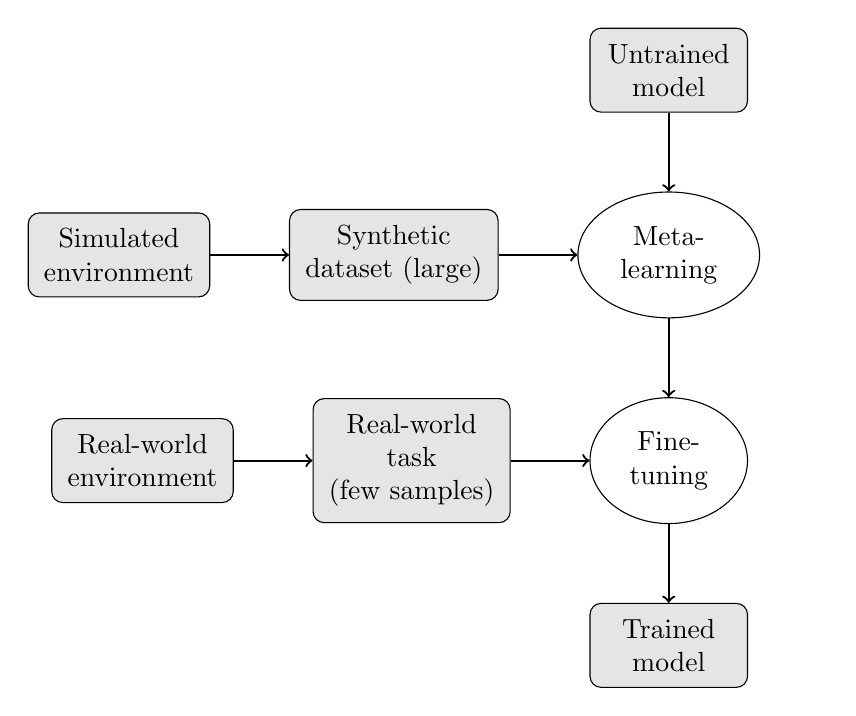
\begin{tikzpicture}
[
inner sep=2mm, 
minimum width=2.0cm, 
minimum height=1.0cm, 
node distance = 1.0cm,
std1/.style={rectangle, rounded corners,fill=gray!20, draw=black, align=center},
std2/.style={rectangle, rounded corners,fill=gray!20, draw=black, align=center},
std3/.style={ellipse, rounded corners,fill=white, draw=black, align=center},
]
\node [std1] (simulator) {Simulated\\environment};
\node [std1, right = of simulator] (synthetic) {Synthetic\\dataset (large)};
\node [std3, right = of synthetic] (meta) {Meta-\\learning};

\node [std1, above = of meta] (model1) {Untrained\\model};

\node [std3, below = of meta] (fewshot) {Fine-\\tuning};
\node [std2, left = of fewshot] (real) {Real-world\\task \\(few samples)};
\node [std2, left = of real] (realworld) {Real-world\\environment};


\node [std2, below = of fewshot] (model2) {Trained\\model};

\draw [->,black,thick] (simulator) -- node[above, midway, yshift=0.5cm]{} (synthetic);
\draw [->,black,thick] (synthetic) -- node[above, midway, yshift=0.5cm]{} (meta);
\draw [->,black,thick] (realworld) -- node[below, midway, yshift=-0.5cm]{} (real);
\draw [->,black,thick] (real) -- node[below, midway, yshift=-0.5cm]{} (fewshot);

\draw [->,black,thick] (model1) -- node[right, midway]{} (meta);
\draw [->,black,thick] (meta) -- node[right, midway]{} (fewshot);

\draw [->,black,thick] (fewshot) -- node[right,midway]{} (model2);
\end{tikzpicture}

\caption{Synthetic meta-learning pipeline}    
\label{pipeline}
\end{figure}
\chapter{Background and Theory}
This chapter will introduce the reader to the necessary information needed to understand the background and theoretical motivations that underpin this thesis. In Section \ref{ML}, the reader will be introduced to the basic concepts required to understand this thesis. The theory mainly involves the terminology and the methodology of training and evaluating machine learning models with a focus on deep neural networks. A reader who is well versed in these areas can skip this section. Section \ref{metalearning} will explain the concepts of meta-learning and few-shot learning and introduce the reader to the \gls{MAML} algorithm and its underlying theory. Section \ref{previous-work} will cover previous research related to synthetic data generation. Section \ref{related-work} will cover some examples of contemporary work that have attempted to solve similar issues related to meta-learning as this thesis. Section \ref{approach} will, in detail, outline the proposed approach. It will also outline the advantages of the suggested approach in comparison to existing methods.

\section{Machine Learning}\label{ML}
Machine learning is a field of study concerned with creating models that learn by utilizing statistics extracted from previously observed data. There are several forms of learning algorithms. \textit{supervised learning} refers to training a model on a set of labelled training data $\mathcal{D} = \{\bm{X}, \bm{Y}\}$ where $\bm{X} = \{\bm{x}_1, \dots, \bm{x}_n\}$ are the input data and $\bm{Y} = \{y_1, \dots, y_n\}$ are \textit{labels} that define the output of the function $F: \mathbb{R}^n \to \mathbb{R}$ the algorithm should learn. The learning is supervised in the sense that the algorithm can inspect the label $y_i$ of each datum $x_i$ to asses how well it performs. This assessment is commonly done by computing a cost (or loss) function, which assesses the disparity between the algorithms guess $\hat{y}_i$, and the true label $y_i$~\cite{deeplearningbook}.

In contrast, \textit{unsupervised learning} refers to the problem of training an algorithm on unlabeled training data. This lack of labeling forces the algorithm to learn and infer properties of the data on its own, without the aid of a supervisor~\cite{deeplearningbook}.

\subsection{Generalization and Overfitting}
The goal of any machine learning algorithm is to be able to generalize well to previously unseen data. Generalization as a concept can be formally defined as the error rate the model or algorithm exhibits on unseen data. A lower error on this test-data implies higher generalization and vice versa~\cite{deeplearningbook}.

Every machine learning model possesses two attributes that relate to its ability to generalize. One is \textit{bias}, expressed as $E[\hat{f}(x) - f(x)]$, which is the difference between the expected prediction of the model and the true value it tries to predict. A model with high bias will \textit{underfit} to the training data, resulting in high training error rates. The reason why is because high bias models are inherently limited in what they can learn, and are restricted to a more narrow problem domain then what the training task requires~\cite{bishop}. 

The other is \textit{variance}, which refers to the expected squared difference between each prediction and the average prediction: $E\Big[(\hat{f}(x) - E[\hat{f}(x)])^2\Big]$. For a model with high variance, small changes in the training data can strongly affect the predictions on the test data. Such a model is sensitive to noise and random patterns in the training data. As a result, it will often \textit{overfit} to training data, showing low error rates during training, while generalizing poorly on the test data~\cite{bishop, deeplearningbook}.

The \textit{bias-variance trade off} is a fundamental concept within machine learning which refers to the relationship between the \textit{bias} and the \textit{variance}. Reducing the variance of a model will invariably result in an increase in its bias, and vice versa. To optimize performance in a model, one needs to find a proper balance between bias and variance. Finding a proper balance can, for example, be done by \textit{regularization}, which entails adding certain restrictions to a high-variance model in order to lower its variance~\cite{bishop}.

\subsection{Deep Learning}
Deep learning is a subfield within machine learning that focuses on the study of \glspl{ANN} and deep architectures. The field has, in recent years, seen a substantial increase in popularity, despite the technology dating back to the 1980s, with the \gls{MLP} and the back-propagation algorithm. Large public datasets, increasingly powerful hardware, as well as increased knowledge of how these models can be trained, have all contributed to its recent rise to popularity~\cite{deeplearningbook}.

%\begin{equation} o =\sum_i(w_i x_i) + b \end{equation}
\tikzset{basic/.style={text width=1em,text badly centered}}
\tikzset{input/.style={basic}}
\tikzset{weights/.style={basic}}
\tikzset{functions/.style={draw, basic,circle}}

\begin{figure}
    \centering
    \begin{tikzpicture}
        \node[functions] (center) {$\alpha$};
        \node[right of=center] (right) {};
            \path[draw,->] (center) -- (right);
        \node[functions,left=3em of center] (left) {$\sum$};
            \path[draw,->] (left) -- (center);
        \node[weights,left=3em of left] (2) {$w_2$} -- (2) node[input,left of=2] (l2) {$x_2$};
        
        
        \node[above=3em of left] (bias) {$b$};
            \path[draw,->] (bias) -- (left);
        
            \path[draw,->] (l2) -- (2);
            \path[draw,->] (2) -- (left);
        \node[below of=2] (dots) {$\vdots$} -- (dots) node[left of=dots] (ldots) {$\vdots$};
        \node[weights,below of=dots] (n) {$w_n$} -- (n) node[input,left of=n] (ln) {$x_n$};
            \path[draw,->] (ln) -- (n);
            \path[draw,->] (n) -- (left);
        
        \node[weights,above of=2] (1) {$w_1$} -- (1) node[input,left of=1] (l1) {$x_1$};
            \path[draw,->] (l1) -- (1);
            \path[draw,->] (1) -- (left);
        \node[weights,above of=1] (0) {$w_0$} -- (0) node[input,left of=0] (l0) {$1$};
            \path[draw,->] (l0) -- (0);
            \path[draw,->] (0) -- (left);
            
    \end{tikzpicture}
    \caption{Single neuron with $n$ inputs and activation function $\alpha$}
    \label{fig:neuron}
\end{figure}

The core of an \gls{ANN} is a basic linear unit called a \textit{neuron}, \textit{node} or \textit{perceptron} (see Figure \ref{fig:neuron}), which is superficially inspired by the neurons in the human brain. These neurons compute the weighted sum of the input vector $\mathbf{x}$ with added an offset called \textit{bias} ($\beta$ in Figure \ref{fig:neuron}). A non-linear activation function is then applied to the output of the neuron ($\alpha$ in Figure \ref{fig:neuron}). The activation function allows the network to express more complex functions than strictly linear ones. This activation function can be any non-linear differentiable function, but the most common function is the \gls{RELU}~\cite{deeplearningbook}.

A set of parallel neurons that are joined together make up a layer. An \gls{ANN} is constructed by stacking several of these layers, by letting the output of one layer become the input to the next layer (see Figure \ref{fig:ann}). The network then takes some input vector $x$, feeds it through each layer in the network, and lets the final layer, the output layer, produce the network's prediction $\hat{y}$. If the task is a classification task, a \textit{softmax} function is often applied to the final prediction vector $\hat{y}$. The softmax function normalizes the values in the vector to a valid probability distribution~\cite{deeplearningbook}.

\def\layersep{3cm}
\begin{figure}[h]
\centering
\begin{tikzpicture}[shorten >=1pt,->,draw=black, node distance=\layersep]
    \tikzstyle{every pin edge}=[<-,shorten <=1pt]
    \tikzstyle{neuron}=[circle,fill=white!25,minimum size=17pt,inner sep=0pt]
    \tikzstyle{input neuron}=[neuron, draw=black, thick];
    \tikzstyle{output neuron}=[neuron, draw=black, thick];
    \tikzstyle{hidden neuron}=[neuron, draw=black, thick];
    \tikzstyle{annot} = [text width=4em, text centered]

    % Draw the input layer nodes
    \foreach \name / \y in {1,...,4}
    % This is the same as writing \foreach \name / \y in {1/1,2/2,3/3,4/4}
        \node[input neuron, pin=left:$x^{1}_\y$] (I-\name) at (0,-\y) {};

    % Draw the hidden layer nodes
    \foreach \name / \y in {1,...,5}
        \path[yshift=0.5cm]
            node[hidden neuron] (H-\name) at (\layersep,-\y cm) {};

    % Draw the output layer node
    \node[output neuron,pin={[pin edge={->}]right:$\hat{y}_1$}, right of=H-3] (O) {};

    % Connect every node in the input layer with every node in the
    % hidden layer.
    \foreach \source in {1,...,4}
        \foreach \dest in {1,...,5}
            \path (I-\source) edge (H-\dest);

    % Connect every node in the hidden layer with the output layer
    \foreach \source in {1,...,5}
        \path (H-\source) edge (O);

    % Annotate the layers
    \node[annot,above of=H-1, node distance=1cm] (hl) {Hidden layer};
    \node[annot,left of=hl] {Input};
    \node[annot,right of=hl] {Output};
\end{tikzpicture}
\caption{Simple ANN with a single hidden layer.}
\label{fig:ann}
\end{figure}

\subsection{Convolutional Neural Networks}
The \gls{CNN} is a specific form of neural network that is specialized in processing grid-like input maps, such as images. A standard \gls{CNN} consists of a set of stacked \textit{convolutional layers}, followed by a set of \textit{fully-connected} layers, similar to a standard neural network. The main building block, the \textit{convolutional layer}, consists of three main components: A set of \textit{kernels}, an non-linear \textit{activation function} and a resolution reducing \textit{pooling layer}~\cite{deeplearningbook}.

The \textit{kernels} (or \textit{filters}) consist of a set of trainable weights that, similarly to the perceptron, apply a linear function to regions in the grid-like input. These regions, also known as receptive fields, are laid out in a grid-like fashion over the input, in order to preserve the input's spatial information. The resulting grid-like output of a kernel is commonly referred to as a \textit{feature-map}. A single layer commonly has a large number of kernels, which each learns to identify some feature in the input~\cite{deeplearningbook}.

The \textit{activation function} is a non-linear function, such as \gls{RELU}, that is applied to the feature-maps outputted by the kernels. Similarly to its use in ANNs, it serves the purpose of allowing the networks to express more complex, non-linear functions. Similarly to ANNs, a common choice for activation function is the \gls{RELU}~\cite{deeplearningbook}.

The \textit{a pooling layer} applies a pooling operator, such as \textit{max} or \textit{mean}, over regions in the feature maps (see Figure \ref{fig:pool}). The pooling layer reduces the overall resolution of the outputted feature maps, while still retaining the essential information. Reducing the dimensionality of the output have the advantage of requiring less trainable weights in later layers, reducing the risk of overfitting~\cite{deeplearningbook}.

\begin{figure}[H]
    \centering
    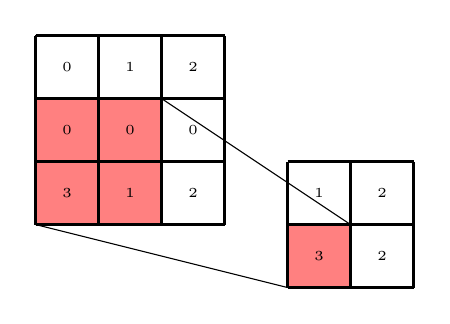
\begin{tikzpicture}[scale=0.8,every node/.style={minimum size=1cm}]
            \draw[fill=white] (-4,0) rectangle (-1,3);            
            \draw[fill=red!50] (-4,0) rectangle (-2,2);
            \draw[draw=black,thick] (-4,0) grid  (-1,3);    
                           
            
            \node (000) at (-3.5,2.5) {\tiny 0};
            \node (001) at (-2.5,2.5) {\tiny 1};
            \node (002) at (-1.5,2.5) {\tiny 2};
            
            \node (010) at (-3.5,1.5) {\tiny 0};
            \node (011) at (-2.5,1.5) {\tiny 0};
            \node (012) at (-1.5,1.5) {\tiny 0};
            
            \node (020) at (-3.5,0.5) {\tiny 3};
            \node (021) at (-2.5,0.5) {\tiny 1};
            \node (022) at (-1.5,0.5) {\tiny 2};
         
         
             
             \draw[fill=white] (0,-1) rectangle (2,0);
            \draw[fill=red!50] (0,-1) rectangle (1,0);            
            \draw[draw=black,thick] (0,-1) grid (2,1);

             \draw (-4,0) -- (0,-1);
             \draw (-2,2) -- (1,0);
                 
            \node (100) at (0.5,0.5) {\tiny 1};
            \node (101) at (1.5,0.5) {\tiny 2};

            \node (110) at (0.5,-0.5) {\tiny 3};
            \node (111) at (1.5,-0.5) {\tiny 2};            
    \end{tikzpicture}
    \caption{Example of Max Pooling}
    \label{fig:pool}
\end{figure}

Some convolutional layers also include an additional component called a \textit{batch-normalization layer}. The batch-normalization layer is a function that scales its input to have zero mean and unit variance, with respect to all inputs in the current mini-batch. This function is most commonly applied before the activation function to make the network learn faster~\cite{batchnorm}.

\subsection{Training Neural Networks}
Feed forward neural networks are trained in a \textit{supervised fashion} where it is presented with data-and-label pairs $(x_i, y_i)$, and aims to minimize a task-specific loss or cost function $\mathcal{L} \rightarrow \mathbb{R}$. This loss function is a measurement of the disparity of the network's guess $f_{\theta}(x_i) \rightarrow \hat{y}_i$ and the ground truth value $y_i$.

The networks are trained using an iterative optimization algorithm, called \textit{gradient descent}. At each iteration, the algorithm computes the gradient of the network using the training data and moves the weights one step proportional to the negative gradient. Moving along the negative gradient can be conceptualized as trying to go down a hill, and at every step walking down the direction which has the steepest slope~\cite{deeplearningbook}.

More formally, if some network is parameterized by $w_t$ at iteration $t$ and the goal is to minimize loss function $L$ then a single step of gradient descent is expressed as:

\begin{equation}
    w_{t+1} = w_{t} - \alpha \partder{L}{w_t}
\end{equation}

Where the \textit{learning rate} $\alpha$ is a \textit{hyperparameter}, a variable that needs to be manually set before training the network. The learning rate defines how big of a step the parameters should move in each iteration. If $\alpha$ is too high, the algorithm will move erratically, often overshooting good local minima. On the other hand, if the learning rate is too low, the algorithm will take too long to converge~\cite{deeplearningbook}.

There exist a set of different versions of gradient descent, each with different approaches to getting an estimate of the current gradient. In \textit{batch gradient descent} the gradient is computed over all the training examples in the training set. Using all data points provides an unbiased estimate of the gradient, but is often computationally expensive to calculate. \textit{Stochastic gradient descent} instead samples a random data point from the training set at each iteration, and uses that single data-point to compute the gradient estimate. This estimate is often noisier than the batch approach but is significantly faster to compute. Lastly, \textit{mini-batch gradient descent} is a combination of the two previous methods. It randomly samples a small \textit{mini-batch} of examples at each update, and uses that mini-batch to compute a less noisy estimate of the gradient estimate~\cite{deeplearningbook}.

The solution space of neural networks is both non-linear and non-convex. Therefore, gradient descent is not guaranteed to reach the global minimum of the loss-function, since the negative gradient can be pointing towards local minima. To counteract this, there exists modifications to the gradient descent algorithms that attempt to use previous knowledge of the solution space to guide the network towards better solutions~\cite{deeplearningbook}. One example of such an algorithm is the \textit{momentum} algorithm, which stores an exponential moving average over all previous gradients. This average is then used as the update direction, rather than the standalone gradient. More formally, the update for a single weight $w_t$ at time $t$ with momentum becomes:

\begin{equation}w_{t+1} = w_{t} - \alpha V_t\end{equation}
where 
\begin{equation}V_t = \beta V_{t-1} + (1-\beta)\partder{L}{w_t}\end{equation}
Here, $\alpha$ is the normal learning rate, and $\beta$ is a manually set hyper-parameter that determines how quickly the old gradients should be forgotten.

Another optimization algorithm is the \textit{Adam} algorithm. In addition to keeping a moving average over past gradients, this algorithm also uses an adaptive learning rate for each individual weight. These adaptive learning rates are calculated using a exponential moving average over past square gradients. More formally, the update for a single weight $w_t$ at time $t$ becomes:

\begin{equation}w_{t+1} = w_t - \frac{\alpha}{\sqrt{\hat{S}_t + \epsilon}} \hat{V}_t\end{equation}
where 
\begin{equation}\hat{V}_t = \frac{V_t}{1-\beta^t_1}\end{equation}
\begin{equation}\hat{S}_t = \frac{S_t}{1 - \beta^t_2}\end{equation}

\begin{equation}V_t = \beta_1 V_{t-1} + (1-\beta_1)\partder{L}{w_t}\end{equation}
\begin{equation}S_t = \beta_2 S_{t-1} + (1 - \beta_2)\left(\partder{L}{w_t}\right)^2\end{equation}

Here, $\alpha$ is the base learning rate, $\epsilon$ is a small value that prevents division by zero, and $\beta_1$ and $\beta_2$ adjust the two moving averages.


\subsection{Data Augmentation}\label{augmentation}
Data augmentation is a common approach to artificially increase training data by applying label invariant transforms to existing data. These transformations are commonly known as augmentation functions. Data augmentation is a standard way in deep learning to reduce overfitting when the amount of actual data is scarce. It can also have the added effect of introducing noise in the training process, which can also help prevent overfitting~\cite{deeplearningbook}.

The choice of augmentation function is highly domain-specific since the transforms that are label invariant varies between domains. For example, rotating an image of a dog 180 degrees does not change its natural class, it still portrays a dog. However, rotating an image containing the digit nine 180 degrees would change its class from nine to six. 

Generally, if one has a set of classes $C_0,...C_{m-1}$ and a set of data points $x_0,...,x_{n-1}$ and an augmentation-function $A$, then one wants $x_i \in C_j, A(x_i) \in C_j$ to hold for the augmentation function~\cite{deeplearningbook}.

Standard augmentation functions for image data include: flipping images horizontally/vertically, rotating images, adding random image noise, and adjusting contrast and saturation~\cite{deeplearningbook}.

\subsection{Transfer Learning}
Transfer learning is a field within machine learning that focuses on utilizing knowledge gained while solving one problem and applying it to a related but different problem. The idea is that for two related tasks, a \textit{source task} and a \textit{target task} there exist an overlap of knowledge that can be extracted from the source task and used to aid in the learning of the target tasks. For example, a person that learns to play the piano will have an easier time to learn playing guitar later, compared to a person who has no prior musical experience. The reason is that there is an overlap in terms of knowledge between the \textit{source task} of learning piano, and the target task of learning guitar, for example reading sheet music, a sense of rhythm and finger dexterity. Transfer learning aims to apply the same logic to machine learning tasks~\cite{transferlearning}.   

A common approach to transfer learning is to extract the first set of layers of a \gls{CNN} trained on a large amount of labeled data, such as the ImageNet dataset~\cite{imagenet}. These first layers output a set of generic mid-level features that are useful for a variety of visual tasks~\cite{cnn-features}. To correct for any difference in distribution between the source and the target domain, a set of additional adaption layers are appended to these extracted layers. These adaption layers are then trained on a small set of labeled data from the target domain, while the previously extracted layers remain locked in place. This approach is called \gls{TCNN} and is one of the most common methods when training deep \gls{CNN}s~\cite{transferlearning}.

\subsection{Multi-Task Learning/Joint Learning}\label{MTL}
Joint Learning or \gls{MTL} is a method of training models that aims to improve the model's ability to generalize by forcing it to learn multiple tasks simultaneously. The model is trained on several distinct but domain-related tasks and aims to reduce the expected cost over all the tasks. The intuition behind this approach is that by forcing a network to learn to use the same input data for different tasks, the network will be forced to have a more general internal feature representation that will prevent overfitting and improve overall performance ~\cite{multi-task-learning}. 

\gls{MTL} for neural networks is done using either \textit{soft} or \textit{hard parameter sharing} of the hidden layers. In hard sharing, the initially hidden layers of the network are shared between all tasks, while each task has a unique set of final output layers. In soft sharing, each task has a unique network, but the difference between the weights in the networks are regularized on a layer by layer basis in order to force the networks to be more similar~\cite{multi-task-learning}.

\section{Few-Shot Learning and Meta-Learning}\label{metalearning}
Few-shot learning is a specific form of machine learning problem, where limits are set on how much data a model is allowed to observe during training. For most machine learning and deep learning tasks, the model is provided an extensive training set from which to learn. In contrast, in few-shot learning tasks, the models are only provided a handful of examples during training, with the number of examples being an integral part of the problem definition~\cite{maml}. 

For classification problems it is common to use the description $N$-way $K$-shot learning, where there are \textit{N} distinct classes and the model is allowed to train using \textit{K} examples from each class. $K$ should be small in order for the task to be considered a few-shot learning tasks. For regression, it is instead common to use the term $K$-shot learning, where $K$ is the total number of data points the model is allowed to observe~\cite{maml}.

%\subsection{Meta-Learning}
Meta-learning, or learning how to learn, is a concept within machine learning that has its origin in the late 1980s~\cite{unsup-maml-rand}. Although the term has been applied to various scenarios throughout the literature, meta-learning generally refers to a training scenario in which a model learns on two different levels. An initial \textit{meta-learning phase} where the model gradually acquires knowledge across various tasks $T_1, ..., T_N$, and a second \textit{meta-testing phase} where the previously meta-trained model is trained on previously unseen tasks $T_{N+1}$ with a limited number of examples~\cite{maml, unsup-maml-rand, santoro}. 

\change{Meta-learning is a common method for tackling few-shot learning problems. The idea is that by having a model meta-train on few-shot learning task, the model can then learn a method of learning, allowing it to quickly learn previously unseen few-shot tasks. 
%A \textit{task} is a very general concept that can be difficult to properly define, but can consist of everything from different forms of classification to reinforcement problems. In its most general form a task can be considered a mapping from some observation $x$ to some output $\textbf{a}$. More formally this can be expressed as
%$T=\{\mathcal{L}(x_1, \textbf{a}_1,...,x_{H}, \textbf{a}_H), q(x_1), q(x_{t+1}|x_t, \textbf{a}_t), H\}$. 
%Here, $q(x_t)$ is the distribution over initial observations. $q(x_{t+1}|x_t, \textbf{a}_t)$ is the transition distribution between observations. $H$ is the number of episodes, which for independently and identically distributed samples is 1. Lastly, $\mathcal{L} \rightarrow R$ is the task-specific loss function used to guide the learning process when it trains using gradient descent.

In order to sample few-shot classification tasks, one needs a large dataset with a large set of classes. As an example, one can consider the Omniglot dataset~\cite{omniglot}. It consists of 1623 different characters from a range of different alphabets, with each character having twenty hand-drawn examples. Sampling 5-way 1-shot classification tasks from this dataset would entail randomly selecting five classes from the complete set of 1623 and taking one example from each class as training data.}

There are many different approaches to meta-learning. One example is memory-augmented neural networks~\cite{santoro}. These recurrent networks have access to an external memory module to which it can read and write freely. The external memory module allows it to quickly encode new information, which in turn makes it very suitable to learn new tasks quickly. 

Another example is meta-networks~\cite{meta-networks}. These networks relies on a concept called \textit{fast} and \textit{slow} weights. The slow weights are updated using normal gradient descent. The fast weights, however, are updated by an external meta-learner module that uses input from both the original model, as well as knowledge of previous tasks, to predict the new weights. The fast and slow weights are then combined in the final prediction~\cite{meta-networks}.

Another approach to meta-learning is \textit{metric learning}. Rather than training a model to learn new tasks, metric learning aims to find a task-invariant similarity metric across the set of training tasks~\cite{siamese}. This metric can then be used classify an entirely new set of classes by comparing the test samples to the labeled training samples. A few examples of these approaches are the Siamese Neural Networks~\cite{siamese} and the Matching Network~\cite{matching}.

\glsreset{MAML} \change{Removed section}
The meta-learning method used in this thesis is \gls{MAML}~\cite{maml}. Unlike most other methods it does not require any specialized model architecture and can be used with any gradient descent trained model. The goal of \gls{MAML} is to find a weight initialization that is optimized for learning new tasks. Finding such a weight initialization can be conceptualized as finding an internal feature representation that generalizes to a broad range of tasks~\cite{maml}. With such a representation, the top-layers of, e.g., a neural network can be fine-tuned to a new task in a couple of gradient steps~\cite{maml}.

\begin{algorithm}[H]
\SetAlgoLined
\SetKwInOut{Input}{Input}
\SetKwInOut{Output}{Output}
\Input{$p(T)$: distribution over tasks}
\Input{$\alpha, \beta$: step size parameters}
Randomly initialize $\bm{\theta}$ \\
\While{\text{not done}} {
    Sample meta-batch of tasks $T_1,...,T_n \sim p(T)$ \\
    where each task $T_i$ contains training data $\mathbf{x}_i$ and validation data $\mathbf{x}'_i$\\
    \ForEach{$T_i$} {
        Update: $\theta_i'  \leftarrow \theta - \alpha \nabla_{\theta} \mathcal{L}_{T_i}(f_{\theta}^{\mathbf{x}_i})$
    }
    Update $\theta \leftarrow \theta - \beta \nabla_{\theta}\sum^{n}_{i=1} \mathcal{L}_{T_i}(f_{\theta'_i}^{\mathbf{x}'_i})$
}
\bo{return } $\theta$ 
\caption{Model-Agnostic Meta-Learning}
\label{alg:maml}
\end{algorithm}

\gls{MAML} is outlined in Algorithm \ref{alg:maml}. Input to \gls{MAML} consist of a distribution over tasks $p(T)$ and a model $f_{\theta}$ parameterized by $\theta$. It also uses two additional hyperparameters: $\alpha$, the learning rate for the inner update step and $\beta$, the learning rate for the outer update step.

During training, a fixed number of tasks $T_i$ are sampled for each meta iterations. The sampled tasks are referred to as a \textit{meta-batch}, and the number of tasks to be sampled during each step is referred to as the \textit{meta-batch size}. 

Each training step in \gls{MAML} is divided into two distinct steps: First, an inner, task-specific update step called the \textit{inner update step}. Second, an outer meta-training step called the \textit{outer update step}. For each task $T_i$ in a meta-batch, a training set $\mathbf{x}_i$ and a validation set $\mathbf{x}'_i$ is sampled. The training set $\mathbf{x}_i$ is used during the inner update step, while the validation set $\mathbf{x}'_i$ is used during the outer update step.

In the inner update step, the the current model parameters $\theta$ are updated using batch gradient descent with the sampled task-specific training data $\mathbf{x}_{i}$ and the task-specific loss $\mathcal{L}_{T_i}$. (To keep the notation simple the number of update steps are limited to 1, but in practice it can be extended to any number of steps.) This update step results in the updated parameters $\mathbf{\theta}'_{i} = \theta- \alpha\nabla_{\theta}\mathcal{L}_{T_i}\left(f_{\theta}^{\mathbf{x}_{i}}\right)$ for each task $T_i$ in the meta-batch. 

In the outer update step, the task-specific loss $\mathcal{L}_{T_i}$ is computed with the task-specific validation data $\mathbf{x}'_{i}$ and the task-specific parameter $\theta_i$ from the inner update step. These losses of all the tasks in the meta-batch are then added together, serving as a measurement on how well $f_{\theta}$ was able to learn the tasks. 

The training objective of \gls{MAML} can be formalized as:
\begin{equation} \min_{\theta} \sum_{T_i \sim p(T)} \mathcal{L}_{T_i}\left(f_{\theta'_i}^{\mathbf{x}'_{i}}\right)\end{equation}

This objective can be interpreted as finding a parameter setting $\theta$ that minimizes the expected loss after the inner update step on all the tasks sampled from the task distribution. Such a parameter setting $\theta$ would mean the model was in a good position to quickly learn a new task. \gls{MAML} uses gradient descent to optimize for this objective, computing the gradient with respect to $\theta$ over the current meta-batch. In practice, a more sophisticated gradient method can also be used, like for example Adam.

\change{Removed a section header}
%\subsubsection{First-Order MAML and Reptile}\label{fomaml}
The outer update step in the \gls{MAML} algorithm requires computing the gradient through a gradient update, which requires the computation of the second ordered Hessian Matrix. Computing the Hessian matrix for a neural network can be computationally expensive and can increase training time significantly. In order to speed up learning it is possible to ignore the second order gradients by considering parameters $\theta'_i$ as constant during the outer update.~\textcite{maml} showed that although this has a slightly negative effect on performance, it will still produce result comparable to the standard \gls{MAML} method. This first-order modification of the \gls{MAML} algorithm is called \gls{FOMAML}.

A modification to the \gls{FOMAML} algorithm called Reptile was later proposed by \textcite{reptile}. Similarly to \gls{FOMAML}, Reptile does not compute the second order gradients of the outer update. However, Reptile takes this one step further by completely ignoring the use of validation data. Instead, it uses the averages of the task-specific weight update $\theta'_i$ to compute the outer update step. 

This approach makes the training more akin to \gls{MTL} (see Section \ref{MTL}) than \gls{MAML}, at least when performing a single update step during training. Averaging over $\theta'_i$  also makes it easier for Reptile to apply more complex optimization methods in the inner-update step, unlike \gls{MAML}, which uses standard gradient descent~\cite{reptile}.

\change{Removed the algorithm}
% \begin{algorithm}[H]
% \SetAlgoLined
% \SetKwInOut{Input}{Input}
% \SetKwInOut{Output}{Output}
% \Input{ $p(T)$ - task distribution}
% \Input{ $\eta$ - step size parameters}
% Randomly initialize weights $\theta$ of model $f_{\theta}$\\
% \While{\text{True}} {
%     Sample tasks $T_1,...,T_n \sim p(T)$ \\
%     \ForEach{$T_i$} {
%         Update $\theta_i$ with some optimizer $U$(e.g. Adam or SGD) \\
%         with respect to loss $\mathcal{L}_{T_i}$: \\
%         $\theta_i'  \leftarrow U_{T_i}(f_{\theta}; \mathcal{L}_{T_i})$ \\
%     }
%     Update $\theta \leftarrow \theta + \eta \frac{1}{n}\sum_{i=1}^{n}(\theta'_i - \theta) $\\
% }
% \bo{return } $\theta$ 
% \caption{Reptile}
% \label{alg:reptile}
% \end{algorithm}


\section{Previous Work}\label{previous-work}
A significant portion of this thesis will focus on the effect of manipulating synthetic data in order to increase the performance of machine learning models. This section will highlight some of the previous works which have utilized synthetic data for training deep learning models, and whose results have influenced the approach used in this thesis.

\subsection{Synthetic Data}
The term \textit{synthetic data} is a very general term that refers to data which have been explicitly generated for a specific learning task, rather than being the by-product of an actual event. Synthetic data is a common approach to tackle one of the most common problems of deep learning: the need for large datasets. The data can be fully synthetic~\cite{domainrand, domainrandcars, object-detection-synth}, meaning no real-world data were used during the generation, or it can be partially synthetic~\cite{cropandpaste}, meaning it uses actual data as a basis.

Synthetic data have been used to train deep learning models for a variety of tasks. Some examples include: object detection ~\cite{domainrand, cropandpaste, domainrandcars, object-detection-synth}, optical flow estimation ~\cite{flying-chairs}, text detection in natural images~\cite{text-detection} and 3D face reconstruction ~\cite{synth-face} to name a few.

An important consideration when using synthetic data, especially image data, is how close to reality the generated images need to be to achieve good results. This topic has been covered extensively in various research. \textcite{object-detection-synth} tested, for the task of object detection, how changing low-level textures in their synthetic images affected model performance. They concluded that the effect of making the images more realistic was negligible, showing that realism might not be important when generating synthetic image data. 

Similarly, both \textcite{domainrand} and \textcite{domainrandcars} were able to train machine learning models with highly unrealistic images by randomizing aspects of their rendering processes when producing the training images.

Lastly, \textcite{goodsynthetic} performed a thorough investigation regarding what kind of synthetic images is the most optimal when training models for optical flow estimation. Their findings were that visual variety is crucial for the model's ability to generalize, while realism has minimal effect on performance. They also concluded that mixing different datasets, like more realistic and more simplistic datasets can also improve performance. Lastly, they concluded that utilizing camera knowledge could be essential. For example, mimicking the lens distortion of the real camera, i.e., the camera that took the test-data, was shown to have a noticeable effect on performance~\cite{goodsynthetic}.

\subsection{Domain Randomization (DR)}
An inherent problem with using approximations of the real world, such as simulations, is that there will always be a disparity between the simulation and the real world. This disparity can be a problem when training deep neural networks since these networks often are sensitive to shifts in the domain. Attempting to reduce this disparity is often time-consuming, requires domain-specific knowledge, and is limited by the capability of modern rendering technology.

\Gls{DR}~\cite{domainrand, domainrandcars} is a more straightforward approach to synthetic image generation that attempts to utilize the strengths of modern rendering software. That is, to create large quantities of diverse, unrealistic imagery, rather than producing a few images with perfect photo-realism. This approach aims to create data that force the model to become more robust to domain changes.  The idea is if the network can learn to perform a task successfully, regardless of the domain, it should also be able to perform the task in the real world since the real world is simply another domain instance~\cite{domainrand}.

Generating such data entails constructing images from a variety of so-called \textit{domains}, or randomized domains, where a new domain is sampled by randomizing certain aspects of the simulation, such as background, lighting, and object textures. The images are often highly unrealistic, but as a result, they tend to be fast and easy to generate.

\textcite{domainrand} used this approach to train a mechanical arm to accurately pick up objects in the real world, by only training it in various virtual, highly unrealistic, domain randomized simulation settings. \textcite{domainrandcars} used a similar approach to generate highly unrealistic imagery as complementary data for the task of real-world car detection. Using this approach, they were able to outperform other synthetic approaches that utilized more photo-realistic imagery. \textcite{domainrandpose} used \gls{DR} for object detection and 6D pose estimation, achieving results rivaling approaches using real data.

\subsection{Structured Domain Randomization (SDR)}
\Gls{SDR} is a modification of standard \gls{DR}. The idea is to incorporate knowledge of the application domain, or the \textit{context}, in the generation process. Incorporating context can allow the model to not only be robust to changes in lighting and textures but also to, for example, learn how to use background information to find small objects. Instead of randomizing the rendering configuration uniformly, as in \gls{DR}, the configurations are sampled along splines, which limits the variety in the generated scene along some dimensions. 

\textcite{structureddomainrandomization} applied this technique to the task of vehicle detection. The \textit{context} is that the test images have been taken using a camera mounted on a car in traffic. During image generation, a setting is selected from a set of predefined options, all of which consist of the main road in which the camera is fixed. After the scene has been sampled, different parts of the scene are randomized and based on that. These randomized factors include the number of lanes in the road, the number of cars on the road, the texture of each car, the lighting and the weather and more~\cite{structureddomainrandomization}.

This approach resulted in better result compared to standard\gls{DR}. A model trained using only \gls{SDR} images was still able to perform well on real, previously unseen data. If real data is used in conjunction with the \gls{SDR} data, it outperforms a model trained using only realistic data with a significant margin~\cite{structureddomainrandomization}. 

\subsection{Summary}
Most previous research in synthetic image generation has concluded that realism is not important~\cite{domainrand, domainrandcars, object-detection-synth, goodsynthetic}. Instead, variations in lighting~\cite{goodsynthetic, domainrand, domainrandcars} and textures~\cite{domainrand, domainrandcars} have been shown to have a positive effect. Others have also shown that utilizing application domain knowledge, either by adjusting the randomization process ~\cite{structureddomainrandomization} or by using camera knowledge, can further improve results~\cite{goodsynthetic}.

Based on this previous research, the best approach seems to be to generate highly varied data, rather than focusing on making the data realistic. However, the problem with these conclusions is that the results may be task-specific and will not generalize well to higher level tasks such as classification or when used with \gls{MAML}. In order to find the optimal approach to synthetic meta-learning, it is essential to evaluate what forms of image variation that have a positive effect on performance. Since lighting have been shown to be important~\cite{goodsynthetic, domainrand, domainrandcars}, while also being easy to adjust in most simulation-software and game-engines, the main focus of this thesis' experiments will be how randomizing aspects of in-game lighting affects performance.

\section{Related Work} \label{related-work}
This section will outline recent research which has attempted to solve the same issue as this thesis: the requirement of large labeled datasets during meta-training.

\glsreset{CACTU}
\glsreset{UMTRA}
\subsection{CACTU}
\Gls{CACTU}~\cite{unsup-maml} is an unsupervised meta-learning algorithm that automatically generates artificial classification tasks from unlabeled data during the meta-training. The algorithm uses various standard methods of clustering to generate artificial class labels for classification tasks. Each unlabeled data example $\mathbf{x}_i$ is first embedded as a high-dimensional feature vector $\mathbf{z}_i$. These embeddings are then grouped into a fixed number of clusters using standard clustering methods, such as k-means. The cluster which embedding $\mathbf{z}_i$ is clustered with is then considered the class label of $\mathbf{x}_i$.  This process is repeated $P$ times, each time with different scaling applied to each dimension of the embeddings in order to create varying cluster-formations. When generating a new task, a partition $p$ is first sampled uniformly from the set of $P$ partitions. A set of classes $c_1,...,c_N$ are then sampled uniformly from the set of clusters in $p$. Then, a set of data points can easily be sampled for each class. Note that the meta-learning tasks consist of the original data $\mathbf{x}_i$, rather than the embeddings $\mathbf{z}_i$ ~\cite{unsup-maml}. The algorithm performs worse compared to supervised \gls{MAML}. For example, for 5-way 5-shot on miniImageNet, \gls{CACTU} achieves $53.97\%$ while supervised \gls{MAML} achieves $62.13\%$.

\subsection{UMTRA}
\Gls{UMTRA}~\cite{unsup-maml-rand} is another unsupervised meta-learning algorithm, which, similarly to CACTU, automatically generates classification tasks from unlabeled data. However, the approach differs significantly from CACTU. Firstly, it modifies the original \gls{MAML} algorithm to perform only $N$-way 1-shot learning during meta-training, rather than $N$-way $K$-shot learning. Then for each training batch, a set of $N$ samples $x_1,...,x_N$ are sampled uniformly from the unlabeled data set. Each sample is assigned one of the $N$ class labels, resulting in a training batch of the form $D_i = (x_1, 1),...,(x_N, N)$. The batch $D_i$ is then used in the inner gradient step of the normal \gls{MAML} algorithm. In order to create the validation batch used in the outer meta-update step with correct class labels, a class-invariant augmentation function (see Section \ref{augmentation}) is applied to the examples in the training batch, resulting in validation batch $D'_i = (x'_1, 1), ...,(x'_N, N)$. The reason why UMTRA's approach to task construction works is because if a data set has a set of natural classes $C$, which is much larger than the number of classes $N$ in the target task, the probability that any of the $N$ randomly chosen samples are from the same natural class $c$ is small enough to be negligible~\cite{unsup-maml-rand}. Similarly to \gls{CACTU}, the algorithm performs worse compared to supervised \gls{MAML}. For 5-way 5-shot on miniImageNet, \gls{UMTRA} achieves $50.73\%$ while supervised \gls{MAML} achieves $62.13\%$.

\section{Thesis Background and Suggested Approach}\label{approach}
This section will describe and motivate the suggested approach as well as why the thesis was written.

\subsection{FOI}
This thesis has been written in collaboration with the \gls{FOI}. \Gls{FOI} is a Swedish government agency responsible for defense-related research that reports to the Swedish Ministry of Defence. One of the goals of using meta-learning, at least for an organization like \gls{FOI} is to be able to build general meta trained models for general tasks, such as vehicle classification or object detection. These meta-trained models could then act as off-the-shelf models that could quickly be adapted to a new task in a matter of minutes using only a handful of real-world examples. 

\subsection{Approach}
The synthetic meta-learning approach outlined in this thesis is straight-forward. It can be summarized as training a neural network using \gls{MAML} while sampling tasks from a large synthetic dataset, in order to train the model how to quickly learn new tasks. 

Creating a dataset from which one can sample few-shot military vehicle classification tasks entails creating a broad set of classes, each with a non-trivial number of examples. For this thesis, the list of classes consists of \gls{VBS3}'s library of vehicle models, with each vehicle model being considered a unique class. For each vehicle model, multiple image samples are then generated within the simulation. The resulting datasets consist of approximately 106,000 images (2357 different classes and roughly 45 samples per class on average). This amount is much larger than other meta-learning datasets, such as miniImageNet~\cite{matching} with 60,000 images (100 classes, each with 600 images per class), and Omniglot~\cite{omniglot} with 32,460 images (1623 classes with 20 image per class).

\change{Removed repetitive text}

Inspired by previous research in synthetic data generation~\cite{goodsynthetic, domainrand, domainrandcars, structureddomainrandomization}, various levels of randomization is also applied to the data. By also introducing variation in the synthetic data, the hypothesis is that the meta-trained model can learn a \textit{domain agnostic feature representation}, i.e. features that can function regardless of application domain. This general feature representation should then allow the model to quickly adapt to new real-world tasks. 

The strength of this approach is tested by tackling the task of \textit{few-shot military vehicle classification}. The choice of task type, as well as the choice of generation tool, \gls{VBS3}, was a consequence of the collaboration with \gls{FOI}, who wanted to focus on a military-oriented task and who also utilize \gls{VBS3} internally for training purposes.




%In order to prevent the trained models from generalizing poorly on the real world data, much care needs to be taken into account when generating the synthetic data. Previous work has shown that randomizing certain parts of synthetic images can have a positive effect since it can force the model to learn more domain agnostic features~\cite{goodsynthetic, domainrand, domainrandcars, structureddomainrandomization}. Therefore, the proposed data generation process utilizes many of the techniques used previously by ~\textcite{domainrandcars} and by ~\textcite{structureddomainrandomization}. These include using realistic contexts, randomizing lighting, randomizing object position, randomizing setting, randomizing contrast, randomizing saturation, and randomizing object textures. 

%Evaluation of the trained models is then done by sampling some few-shot classification tasks from a small real-world dataset, which has been collected specifically for this thesis. This dataset consists of images of military vehicles gathered from Google and Bing.

\subsection{Why Synthetic Data?}\label{why-synthetic}
The primary reason for why the combination of synthetic data and meta-learning is a promising concept is that it removes the need for a large labeled dataset during the initial metaphase. However, methods like UMTRA ~\cite{unsup-maml-rand} and CACTU~\cite{unsup-maml} (see Section \ref{related-work}) have with relative success been able to train meta-learning models without any use of labeled data. Their success raises the question of why the synthetic approach should be investigated in the first place. 
There are several benefits to using synthetic data for meta-learning when compared to the unsupervised approaches. One is the amount of control it gives over the data. The synthetic data can be coupled with lots of additional information other than class labels, which can be useful when analyzing how well a model learns. One example is the bitmap, which shows what pixels that contains the object of interest. The bitmap can be used in combination with transparent AI techniques, such as GradCam~\cite{gradcam}, to see how well the model learns to focus on the object of interest during training. Synthetic data also makes it possible to adjust how difficult the sampled tasks should be by adjusting how visually similar all samples of a class should be. Changing the structure of a task and a dataset could offer additional insight into how algorithms like \gls{MAML} learn.

Another benefit is the number of possible tasks the process can generate and learn, compared to unsupervised approaches. Methods like UMTRA and CACTU are both limited to generating classification tasks because of how the algorithms approach automatic labeling. Since the \gls{MAML} algorithm can be applied to both classification, regression, and reinforcement learning tasks~\cite{maml}, this seems needlessly limiting. In contrast, the synthetic approach can be configured to generate tasks of any kind, as long as the labeling can be extracted from the simulation.
\chapter{Methodology}
This chapter will outline the methods and techniques used to implement and evaluate the experiments of this thesis. The experiments can be divided into two distinct steps: data generation, where a synthetic dataset is constructed, and the meta training where the model is meta-trained on the synthetic data and then tries to adapt to a set of real-world tasks. Section \ref{image-gen} will cover the image generation process. Section \ref{meta-section} will cover the meta training set up and the training of the neural networks. The following two sections, Sections \ref{software} will outline the software tools used in the experiments.

\section{Data Generation}\label{image-gen}
This section will describe the procedure used to generate synthetic training data from \gls{VBS3}. It will outline how environments and objects are manipulated in the simulator in order to create realistic imagery and how meta-information is extracted from the simulator during generation. Also, this section will list the different adjustable parameters in the data generation setup and how changing these influences the quality and characteristics of the generated data.

\subsection{VBS3}
The tool used for generating image data was the Virtual Battlespace 3 (VBS3) version 18.3.3.8. \gls{VBS3} is a desktop tactical trainer and mission rehearsal software system developed by Bohemia Interactive Simulations. This software is used by many major military organizations, including the U.S. Army and the U.S. Marine. VBS3 has a large library of over 10,000 high-resolution models. This large amount of models makes it useful for generating image data for a variety of semi-realistic military-related tasks, such as generating vehicle images.

The VBS3 software can be controlled through its graphical user interface or via its internal scripting API. %The scripting API uses Bohemia Interactive Simulations own scripting language called \gls{SQF}.


\subsection{Generation Process}
The image generation process is started by initializing the simulation with a fixed setting and a list of vehicles. The setting is chosen from the available library of terrain maps. There are five different standard environments available in VBS3 (see Section \ref{settings}). For the vehicle classification tasks, a list of 2357 vehicle models is used. These classes were extracted by iterating over the list of vehicle models in the VBS3 documentation. These vehicles include everything from large military vehicles like tanks, airplanes, and aircraft carriers to smaller objects like remote controlled cars and drones. 

After a setting is decided the simulator starts iterating over the provided list of vehicle models. For each vehicle, it will take a fixed number of images. Since the task of interest is standard image classification, only a single object at the time is spawned, although the process is easily extended to many objects. After all images of all vehicles have been taken, the simulation will be restarted with a new setting.

The process of generating an image starts by spawning an instance of the current model in a random location in the in-game map. Similarly to ~\textcite{structureddomainrandomization}, the context of the object and setting are taken into account when generating the images. Vehicles that are based in water, like boats, are more likely to be spawned in a body of water. Flying vehicles like drones, planes, and helicopters are either spawned between 2 to 20 meters in the air or spawned laying on the ground. All other land-based vehicles are always spawned standing on the ground in the most realistic way possible. 

After the vehicle has been position in the world, an in-game camera is randomly positioned around the object. The camera is positioned in such a way that the object of interest is clearly visible and not obfuscated completely by the terrain. The distance between the camera and the object is dependent on the size of the objects. For smaller objects like drones, remote-controlled vehicles and smaller boats, the camera is set to be at the most 15 meters from the object. For larger vehicles like transport planes or oil tankers, the camera is given a larger offset, starting from 30 meters to ensure that the object never covers the entire image.

After the in-game camera has found a clear view of the object, the world's lighting and weather effects are randomized, as well as other settings, in order to introduce variance in the images. The camera then takes a photo of the resulting scene, which will be used as training data. Additional meta information, like the current rotation of the object, is also saved. 

After the first photo has been taken, all lighting and weather effects are temporarily disabled in order to create a clearer image. A render mask is then applied to the object, transforming it into a single uniform segment of an easily identified color, such as pink (see Figure. \ref{fig:rendermask}). A second photo is then taken with the same camera as before.

\begin{figure}[H]
\centering
\subcaptionbox{Generated Image}
  {\includegraphics[height=4.4cm]{images/vbs3/bbox/example2.jpg}}
\subcaptionbox{Masked Object}%
  {\includegraphics[height=4.4cm]{images/vbs3/bbox/example2-pink.jpg}}
%\subcaptionbox{Extracted Bounding Box}%
%  {\includegraphics[height=4.4cm]{images/vbs3/bbox/example2-bbox.jpg}}
\caption{}
\label{fig:rendermask}
\end{figure}

Segmentation information and bounding box information is then extracted using the render-masked image. There are several advantages of having access to segmentation information, even if the final target task will not utilize it. It allows for automatic and precise cropping of the object of interest. It also makes it possible to detect bad image samples where the object is hidden or obscured. The simulator, \gls{VBS3}, is not always able to find perfectly suitable camera-angles. Sometimes vegetation and other objects can cover the object. In this thesis, images with an object segment of fewer than 750 pixels were therefore removed in a separate filtering step in order to remove obscured objects. However, this also meant that some of the smaller vehicles had a higher probability of being removed. As a result, some of the classes consisted of fewer images than others.

Between each photo of the same vehicle, the vehicle is moved to a new position within a hundred-meter radius of the previously used position. This range limit is set to allow the simulation to load the background textures properly before the image is taken. If the vehicle is allowed to move over a larger area, the simulation can have a problem loading the background textures with the highest resolution in time, resulting in poor image quality.

This generation process is re-run one time for each of the five available maps, in order to create a high degree of variety in the dataset.

\subsection{Image Randomization}\label{randomization-settings}
The experiments of~\textcite{domainrand},~\textcite{domainrandcars} and~\textcite{structureddomainrandomization} have shown that the variation of the training data can have a substantial effect on the final performance of models trained with synthetic data. Since these methods have never been tested in a meta-learning setting, it is, therefore, essential to determine if the same principles still hold.

In order to investigate this, the simulation setup has been built to allow for certain simulation parameters to be enabled and disabled, which changes how the scenes are randomized. These parameters are: 

\begin{itemize}
    \item \textbf{Context}: Objects are spawned in scenarios that take their real-world context into account (see Figure \ref{with-context}). For example planes and helicopters are spawned in the air, while boats are spawned in bodies of water. Disregarding the context makes the data-generation more akin to standard \gls{DR}, where vehicles can be in any scenario, in any possible position, thus increasing the difficulty of the generated tasks (see Figure \ref{no-context}).
    
    \begin{figure}[H]
    \centering
      {\includegraphics[height=2.4cm, width=3.4cm]{images/vbs3/random-pos/context1}}
      {\includegraphics[height=2.4cm, width=3.4cm]{images/vbs3/random-pos/context2}}
      {\includegraphics[height=2.4cm, width=3.4cm]{images/vbs3/random-pos/context3}}
    \caption{With context enabled}
    \label{with-context}
    \end{figure}

    \begin{figure}[H]
    \centering
      {\includegraphics[height=2.4cm, width=3.4cm]{images/vbs3/random-pos/no-context1}}
      {\includegraphics[height=2.4cm, width=3.4cm]{images/vbs3/random-pos/no-context2}}
      {\includegraphics[height=2.4cm, width=3.4cm]{images/vbs3/random-pos/no-context3}}
    \caption{With context disabled}
    \label{no-context}
    \end{figure}

    \item \textbf{Color Scheme/Texture Randomization}: For a subset of the vehicles (around 800), a randomized color is applied to each editable part of the vehicle. Randomizing the textures is a similar approach to what is done both by~\textcite{domainrandcars, structureddomainrandomization}.
    
    \begin{figure}[H]
    \centering
      {\includegraphics[height=2.4cm, width=3.4cm]{images/vbs3/color-scheme/car/example4-1.jpg}}
      {\includegraphics[height=2.4cm, width=3.4cm]{images/vbs3/color-scheme/car/example4-2.jpg}}
      {\includegraphics[height=2.4cm, width=3.4cm]{images/vbs3/color-scheme/car/example4-3.jpg}}
      
      {\includegraphics[height=2.4cm, width=3.4cm]{images/vbs3/color-scheme/bike/example4-4.jpg}}
      {\includegraphics[height=2.4cm, width=3.4cm]{images/vbs3/color-scheme/bike/example4-5.jpg}}
      {\includegraphics[height=2.4cm, width=3.4cm]{images/vbs3/color-scheme/bike/example4-6.jpg}}
      
        {\includegraphics[height=2.4cm, width=3.4cm]{images/vbs3/color-scheme/plane/example4-7.jpg}}
      {\includegraphics[height=2.4cm, width=3.4cm]{images/vbs3/color-scheme/plane/example4-8.jpg}}
      {\includegraphics[height=2.4cm, width=3.4cm]{images/vbs3/color-scheme/plane/example4-9.jpg}}
    \caption{Different vehicle models with different color scheme}
    \label{color-scheme}
    \end{figure}
    
    \item \textbf{Lighting}:~\textcite{domainrandcars} showed that variations in lighting could have a huge effect on performance. Outlined here are the different methods for randomizing lighting in the simulation. Examples of their combined effect can be seen in Figure \ref{lighting-example}.

    \begin{itemize}
        \item \textbf{Time}: The time of the day is randomly chosen between the range of hours in which the sun is still visible. Changing the internal time results in the sun, the main lighting source, being in various positions, resulting in both different degrees of lighting intensity as well as different shadow shapes (see Figure \ref{rand-time}). 
        \begin{figure}[H]
        \centering
        \subcaptionbox{}
          {\includegraphics[height=2.4cm, width=3.4cm]{images/vbs3/random-light/time/time-0.png}}
        \subcaptionbox{}%
          {\includegraphics[height=2.4cm, width=3.4cm]{images/vbs3/random-light/time/time-3.png}}
        \subcaptionbox{}%
          {\includegraphics[height=2.4cm, width=3.4cm]{images/vbs3/random-light/time/time-5.png}}
        \caption{Randomized Time}
                \label{rand-time}
        \end{figure}
    
        \item \textbf{Crepuscular Rays}: This setting adjusts the color of light rays coming from the in-game sun, as well as the transparency of these rays. Randomizing this configuration results in a high degree of color variation in the images, but can also make the images blurrier (see Figure \ref{rand-rays}). 
     
        \begin{figure}[H]
        \centering
        \subcaptionbox{}
          {\includegraphics[height=2.4cm, width=3.4cm]{images/vbs3/random-light/ray/rays-0.png}}
        \subcaptionbox{}%
          {\includegraphics[height=2.4cm, width=3.4cm]{images/vbs3/random-light/ray/rays-1.png}}
        \subcaptionbox{}%
          {\includegraphics[height=2.4cm, width=3.4cm]{images/vbs3/random-light/ray/rays-4.png}}

        \caption{Randomized Ray Color using VBS3's God Rays}
                \label{rand-rays}
        \end{figure}
     
        \item \textbf{Weather}: With a given probability random weather configurations are chosen. The weather is configured using three variables, level of rain, level of fog, and level of overcast (see Figure \ref{rand-weather}).
 
        \begin{figure}[H]
        \centering
        \subcaptionbox{}
          {\includegraphics[height=2.4cm, width=3.4cm]{images/vbs3/random-light/weather/weather-0.png}}
        \subcaptionbox{}%
          {\includegraphics[height=2.4cm, width=3.4cm]{images/vbs3/random-light/weather/weather-1.png}}
        \subcaptionbox{}%
          {\includegraphics[height=2.4cm, width=3.4cm]{images/vbs3/random-light/weather/weather-3.png}}
        \caption{Randomized Weather}
                \label{rand-weather}
        \end{figure}
             
    \end{itemize}

\end{itemize}


\begin{figure}[H]
\centering
\subcaptionbox{}
  {\includegraphics[height=2.4cm, width=3.4cm]{images/vbs3/realistic-lighting/light-variation/1.png}}
\subcaptionbox{}%
  {\includegraphics[height=2.4cm, width=3.4cm]{images/vbs3/realistic-lighting/light-variation/2.png}}
\subcaptionbox{}%
  {\includegraphics[height=2.4cm, width=3.4cm]{images/vbs3/realistic-lighting/light-variation/3.png}}
\subcaptionbox{}
    {\includegraphics[height=2.4cm, width=3.4cm]{images/vbs3/realistic-lighting/light-variation/8.png}}
\subcaptionbox{}%
  {\includegraphics[height=2.4cm, width=3.4cm]{images/vbs3/realistic-lighting/light-variation/car/1.png}}
\subcaptionbox{}%
  {\includegraphics[height=2.4cm, width=3.4cm]{images/vbs3/realistic-lighting/light-variation/car/2.png}}
\subcaptionbox{}%
  {\includegraphics[height=2.4cm, width=3.4cm]{images/vbs3/realistic-lighting/light-variation/car/3.png}}
\subcaptionbox{}%
  {\includegraphics[height=2.4cm, width=3.4cm]{images/vbs3/realistic-lighting/light-variation/car/4.png}}
\caption{Examples of randomized lighting configurations}
\label{lighting-example}
\end{figure}

\subsection{Generated Datasets} \label{dataset-summary}
In order to evaluate how different randomization settings affects final performance, seven datasets were generated with one or more of the image randomization settings turn on or off. The settings include: \textit{crepuscular Rays, weather, time, context} and \textit{texture} randomization. If \textit{Crepuscular Rays/God Rays} was enabled, the simulation light in each image would be shifted into a random color. If \textit{Weather} was enabled the weather of the simulation was randomized for each photo. If \textit{Time} was enabled, the sun was randomly positioned somewhere in the sky. If \textit{Context} was disabled, the vehicles were positioned without any regard to how their real-world counterparts would behave, while if it was enabled the vehicles were positioned realistically. If \textit{Texture} was enabled, the texture of the vehicles was randomized in each image. These settings have been outlined in further detail in Section \ref{randomization-settings}.

All possible parameter configurations were not tested due to time constraints. For a full outline of all the generated datasets, see Table~\ref{rand-table1}. A \checkmark indicates that that randomization factor was active during the generation of that dataset, while \xmark ~indicates the setting was disabled.

Lighting was hypothesized to be the most critical factor in the generation process since it had previously been shown to have a significant effect on other tasks \cite{domainrand, goodsynthetic}. The first five datasets D1--D5 was therefore constructed to test the combined and individual effect of each light-setting. D1 tests the combined effect of all light settings, while D2 tests how completely static light effects performance. D3--D5 tests the effect of disabling of of the light parameters, in order to see their individual contribution. The last two, D6 and D7, were constructed to test if further randomization with positioning and textures could further improve accuracy.

\begin{table}[h]
\caption{Randomization configurations for the datasets}
\resizebox{\textwidth}{!}{%
  \begin{tabular}{cccccc}
  \hline
    \textbf{Dataset}  & Crepuscular Rays & Weather & Time  & Context & Texture\\
    \hline
    D1      & \checkmark     & \checkmark     & \checkmark  & \checkmark &  \xmark \\
    D2      & \xmark         & \xmark         & \xmark      & \checkmark &  \xmark \\
    D3      & \xmark         & \checkmark     & \checkmark  & \checkmark &  \xmark \\
    D4      & \checkmark     & \xmark         & \checkmark  & \checkmark &  \xmark \\
    D5      & \checkmark     & \checkmark     & \xmark      & \checkmark &  \xmark \\
    D6      & \checkmark     & \checkmark     & \checkmark  & \checkmark &  \checkmark \\
    D7      & \checkmark     & \checkmark     & \checkmark  & \xmark & \xmark \\
    \hline
  \end{tabular}}
  \label{rand-table1}
\end{table}

Since invalid image samples are filtered out after the generation process, there is not a fixed number of samples per class, and the number could vary depending on how small and likely to be obscured the vehicle models were. Similarly, some of the classes were removed if the number of samples was insufficient to sample training samples from. The exact number of data-samples per class can be seen in Table \ref{datasets}.


\begin{table}[h]
\caption{Synthetic dataset statistics}
\label{datasets}
\begin{tabular}{lSSS}
        \hline
        Dataset & \text{\# of classes} & \text{Avg. \# per class} & \text{Total}
        \\\hline        
        D1 & 2357 & 45.14806958 &    106414
        \\ 
        D2 & 2357 & 46.0767925329  &    108603
        \\ 
        D3 & 2358 & 46.0843935539  &    108667
        \\ 
        D4 & 2356 & 45.318336163  &    106770
        \\ 
        D5 & 2357 & 45.14806958  &     106414
        \\ 
        D6 & 2357 & 45.0377598642  &    106154
        \\ 
        D7 & 2342 & 48.1011955594  &    112653
        \\\hline
 \end{tabular}
\end{table}


\subsection{Summary}
The image generation process consists of: for each map and each vehicle model, randomly position the vehicle in the world, randomly position the camera around it, randomize parts of the scene, take an image and save it along with meta-information about the scene. 

The generation process had five parameters that could be adjusted in order to change how the images were randomized. To test the effect of the different parameters, seven different parameter configurations were selected and used to generate datasets containing over 106,000 images.

\section{Meta Training}\label{meta-section}
After a synthetic dataset with the desired properties have been generated, the data was used to train a model using \gls{MAML}~\cite{maml} (see Section \ref{maml}). After the training was finished, the model's performance was evaluated on a set of real-world tasks. This section will outline the setup and methods that were used when training and evaluating the models.

\subsection{Task Generation}\label{task-generation}
One of the most fundamental aspects of methods like \gls{MAML}~\cite{maml} is sampling from a task distribution $p(T)$. A task is sampled from a dataset by first uniformly sampling a set of $N$ classes without replacement from the list of classes in the dataset. A set of training and validation samples are then sampled from the selected classes (see Section \ref{maml} and Algorithm \ref{alg:maml}) without replacement and any overlap.

\subsection{Problem Settings}
For this thesis, three problem settings were explored: 5-way 1-shot, 5-way 5-shot and 5-way 10-shot classification. The 1-shot and 5+shot task utilized regular \gls{MAML} during meta-training. The 10-shot task used \gls{FOMAML} instead of regular \gls{MAML}, since regular \gls{MAML} consumed to much video-memory for that many samples. For all of tasks, a meta-batch size of four and five gradient update steps was used. Ten validation images per class were used for each task. These settings were chosen primarily as a result of hardware limitations since increasing the meta-batch size exhausted the GPU's memory resources, while setting a lower meta-batch size and lowering the number of update steps slowed down training significantly.

\subsection{Image Pre-Processing}
For each image in each task, a square area around the object of interest was cropped. The crop was always performed such that the entire object is contained within the selected region, but is randomly readjusted as not to have the object be in the center. The cropped region was then re-sized to a resolution of 128x128 using bilinear interpolation. The resulting resolution was significantly larger compared to other common meta-learning tasks like Omniglot~\cite{omniglot} or miniImageNet~\cite{matching}. This size was chosen in order to preserve as much detail of the object as possible, in order to allow the model to distinguish between superficially similar objects like different kinds of tanks or different kinds of cars.

\subsection{Image Augmentation}
Data augmentation methods were also applied to all images during the meta-learning phase. These methods were chosen because they have been previously shown to be useful when training with synthetic data ~\cite{structureddomainrandomization}. These methods include:

\begin{itemize}
    \item \textbf{Random Flipping}: Images were flipped horizontally with a 50\% chance.
    \item \textbf{Random Contrast}: The contrast of the images was randomized between 60\% and 115\% of the original contrast.
    \item \textbf{Random Saturation}: The saturation of the images was randomized between 60\% and 150\% of the original image saturation.
\end{itemize}

\subsection{Network Architecture \& Hyperparameters}
The network architecture used in this thesis was the same architecture utilized by ~\textcite{maml} in their experiments with Convolutional Neural Networks. The network consisted of five convolutional layers with 32 convolutional filters with a receptive field size of $3\times3$ and with stride 1. Each convolutional layer used \gls{RELU} activation and was followed by a $2\times2$ max-pooling layer. Batch normalization was also applied between the convolutional operation and the \gls{RELU} activation in each convolutional layer. Lastly, a single, fully connected layer with softmax activation was used to output the final prediction vector.

During meta training the inner learning rate $\alpha$ was set to 0.01. The outer update is performed using Adam with a learning rate of $\beta =0.001$ and additional parameters being set to $\beta_1=0.9, \beta_2=0.999, \epsilon=1e-08$.

The same network was used for all the tasks, with the exception being the final fully connected layer being changed when the number of classes is changed.

\subsection{Test Data}\label{test data}
In order to evaluate the generalizing performance of the models, a small number of real-world images were collected from various sources on the internet. The collected dataset was manually labeled and consist of 42 different object classes with between 15 to 30 images per class. The classes consist of different kinds of military vehicles, such as tanks, boats, airplanes, helicopters, and motorbikes, where each class is a specific vehicle model, for example, JAS Gripen (see Figure \ref{real-images} for examples). %Most of these vehicles do not have a model counterpart in any of VBS3 Datasets. This choice of using mostly new validation classes was made to highlight this approach's ability to generalize to new classes, while also bridging the reality gap.

% Real Images
\begin{figure}[H]
\centering
\subcaptionbox{}
  {\includegraphics[height=2.4cm, width=2.4cm]{images/real-images/helicopter/1.png}}
\subcaptionbox{}%
  {\includegraphics[height=2.4cm, width=2.4cm]{images/real-images/helicopter/2.jpg}}
\subcaptionbox{}%
  {\includegraphics[height=2.4cm, width=2.4cm]{images/real-images/helicopter/3.png}}
\subcaptionbox{}
  {\includegraphics[height=2.4cm, width=2.4cm]{images/real-images/helicopter/4.jpg}}
\subcaptionbox{}%
  {\includegraphics[height=2.4cm, width=2.4cm]{images/real-images/helicopter/5.jpeg}}

\subcaptionbox{}
  {\includegraphics[height=2.4cm, width=2.4cm]{images/real-images/tank/1.jpg}}
\subcaptionbox{}%
  {\includegraphics[height=2.4cm, width=2.4cm]{images/real-images/tank/2.jpg}}
\subcaptionbox{}%
  {\includegraphics[height=2.4cm, width=2.4cm]{images/real-images/tank/3.jpg}}
\subcaptionbox{}
  {\includegraphics[height=2.4cm, width=2.4cm]{images/real-images/tank/4.jpg}}
\subcaptionbox{}%
  {\includegraphics[height=2.4cm, width=2.4cm]{images/real-images/tank/5.jpg}}

\subcaptionbox{}
  {\includegraphics[height=2.4cm, width=2.4cm]{images/real-images/plane/1.png}}
\subcaptionbox{}%
  {\includegraphics[height=2.4cm, width=2.4cm]{images/real-images/plane/2.jpg}}
\subcaptionbox{}%
  {\includegraphics[height=2.4cm, width=2.4cm]{images/real-images/plane/3.jpg}}
\subcaptionbox{}
  {\includegraphics[height=2.4cm, width=2.4cm]{images/real-images/plane/4.jpg}}
\subcaptionbox{}%
  {\includegraphics[height=2.4cm, width=2.4cm]{images/real-images/plane/5.jpg}}

\subcaptionbox{}
  {\includegraphics[height=2.4cm, width=2.4cm]{images/real-images/water/1.jpg}}
\subcaptionbox{}%
  {\includegraphics[height=2.4cm, width=2.4cm]{images/real-images/water/2.jpg}}
\subcaptionbox{}%
  {\includegraphics[height=2.4cm, width=2.4cm]{images/real-images/water/3.jpg}}
\subcaptionbox{}
  {\includegraphics[height=2.4cm, width=2.4cm]{images/real-images/water/4.jpg}}
\subcaptionbox{}%
  {\includegraphics[height=2.4cm, width=2.4cm]{images/real-images/water/5.jpg}}
\caption{Examples of real world images}
\label{real-images}
\end{figure}


\subsection{Performance Evaluation}
After a model had been trained using \gls{MAML} on a synthetically generated dataset, the model's ability to adapt to a real-world task was evaluated. From the dataset described in Section \ref{test data}, tasks were sampled in the same fashion as outlined in Section \ref{task-generation}. The models were given the same number of samples for each class as was defined by the few-shot classification task it was meta-trained on. Then the model was updated using batch gradient descent with a learning rate of 0.01, same as during meta-training. 

Five-thousand tasks were randomly sampled for evaluation, and the models are trained with ten gradient steps for each task. The mean of the model's accuracy after the final update-step, over five-thousand tasks, was then reported as the final accuracy.

\subsection{Baselines}
For this thesis, two baselines were chosen: First, a baseline model named BL1. This baseline involved training the same network used in all other settings, using only the meta-test data, without doing the meta-trained. This baseline was used to give an indication both how difficult the final tasks were to perform and how well the \gls{MAML} algorithm improves performance.

Secondly, a second baseline model was trained using a hand-labeled real-world dataset, collected from Bing and Google Image Search. This baseline was named BL2 and was used to highlight how the synthetic performs in comparison to models trained on real-world data. Its training set consists of 61 different vehicles, with each class consisting of between 80 to 350 RGB images. In total, the number of images is 9954.

\change{Moved to discussion}

\subsection{Summary}
The experiments consisted of training a six-layer \gls{CNN} using \gls{MAML} for each of the seven synthetic datasets (see Table \ref{datasets}). Also, two baselines were trained, one where no pre-training was used (BL1), and one that was trained using \gls{MAML} on a real-world dataset (BL2). Their performance was evaluated by sampling five-thousand tasks from a real-world test dataset and having the networks adapt to each task and then calculating the average accuracy.

\section{Programming Libraries and Frameworks} \label{software}
A mix of Python 3.7+ and the \gls{SQF} scripting language was used to generate the images in VBS3. 

\gls{SQF} is a scripting language developed by Bohemia Interactive Simulations and is used for scenario scripting within the simulation. In this thesis, it was the primary tool for controlling the simulation process, creating scenes, spawning, and iterating over objects and collection and outputting relevant vehicle information.

All other code relating to both the image generation post-processing and all the machine learning code was written in Python 3.7+. Python is a high-level scripting language with a large user-base within the machine learning community, making it the obvious choice for most things machine learning. 

Google's Tensorflow~\cite{tensorflow} library was used to construct machine learning models. Tensorflow is an open source software library developed for high-performance numerical computation. It is used both within the industry and for research applications. The implementation of the meta-learning algorithm was built using Tensorflow 1.10.0 with GPU support.

Nvidia Docker was used to constructing a virtual environment where requirements already installed to run the Tensorflow program efficiently with full GPU support. Docker is a self-contained light-weight virtual machine for which a pre-defined \textit{image} with necessary software dependencies can be installed. A copy of the docker image used to run these experiments will be made available to allow the experiments in this thesis to be easily reproduced.
\chapter{Result}
This chapter presents the results of the experiments outlined in the previous chapter. It will begin by showing the randomization configurations used for each generated dataset. It will then display the accuracy and standard deviation of each of the models trained with one of the datasets, as well as the baselines. Lastly, the meta-training accuracy of the different datasets will be presented.

\section{Datasets}
Table \ref{rand-table} outlines which of the possible randomization options that were enabled or disabled for each of the generated datasets. A full explanation of all settings can be found in Section \ref{dataset-summary}.


\begin{table}[h]
\caption{Randomization configurations for synthetic datasets}
\label{rand-table}
\resizebox{\textwidth}{!}{%Fas
  \begin{tabular}{cccccc}
  \hline
    \textbf{Dataset}  & Crepuscular Rays & Weather & Time  & Context & Texture\\
    \hline
    D1      & \checkmark     & \checkmark     & \checkmark  & \checkmark &  \xmark \\
    D2      & \xmark         & \xmark         & \xmark      & \checkmark &  \xmark \\
    D3      & \xmark         & \checkmark     & \checkmark  & \checkmark &  \xmark \\
    D4      & \checkmark     & \xmark         & \checkmark  & \checkmark &  \xmark \\
    D5      & \checkmark     & \checkmark     & \xmark      & \checkmark &  \xmark \\
    D6      & \checkmark     & \checkmark     & \checkmark  & \checkmark &  \checkmark \\
    D7      & \checkmark     & \checkmark     & \checkmark  &  \xmark & \xmark \\
    \hline
  \end{tabular}}
\end{table}


\begin{table}[h]
\centering
\caption{Test-accuracy in \% for each dataset on \textbf{5-way 1-shot} classification over 5000 test-tasks}
\label{accfiveone}
\begin{tabular}{l *{3}{S}}
        \hline
        Dataset & \text{Mean (\%)} & \text{Std. (\%)} & \text{CI $\pm95\%$}
        \\
        \hline
        BL1  & 31.9468321028136 & 8.0587001344171652 &  \pm 0.2233757712937365
        \\
        BL2  & 62.9369854927063 & 12.306884676218033 & \pm  0.3411294426769018
        \\
        D1  & 46.405258774757385 & 10.25920882821083 & \pm  0.2843707799911499
        \\
        D2  & 37.87154257297516 & 9.331290423870087 & \pm  0.2843707799911499        
        \\
        D3  & 36.92753314971924 & 9.154894948005676 & \pm  0.25376074481755495
        \\
        D4  & 41.715073585510254 & 9.66532900929451 & \pm  0.2679092576727271
        \\
        D5  & 46.327099204063416 & 10.632327944040298 & \pm  0.29471309389919043
        \\        
        D6  & 43.797504901885986 & 9.575874358415604 & \pm  0.26542970445007086
        \\
        D7  & 44.011953473091125 & 10.048750042915344 & \pm  0.2785371383652091
        \\ \hline   
    \end{tabular}
\end{table}

\begin{table}[h]
\centering
\caption{Test-accuracy in \% for each dataset on \textbf{5-way 5-shot} classification over five-thousand test-tasks}
\label{accfivefive}
\begin{tabular}{l *{3}{S}}
    \hline
    Dataset & \text{Mean (\%)} & \text{Std. (\%)}  & \text{CI $\pm95\%$}
    \\\hline
    BL1  & 49.92594717554718 &     9.111414172566245 &     \pm 0.2525561371756853
    \\
    BL2  & 72.88147211074829 &   10.564619302749634 &     \pm 0.2928362926468253
    \\
    D1 & 67.83030033111572 &    9.793011099100113 &     \pm 0.2714484231546521
    \\
    D2   & 59.50989127159119 &    9.523329138755798 &    \pm 0.2639732090756297
    \\
    D3   & 62.06099987030029 &    9.490425884723663 &    \pm 0.26306118816137314
    \\
    D4   & 65.76035618782043 &    9.420520067214966 &    \pm 0.26112350169569254
    \\
    D5   & 69.03369426727295 &    9.92111787199974 &     \pm 0.27499934658408165
    \\
    D6   & 67.11101531982422 &    10.139784216880798 &    \pm 0.28106047903736975
    \\
    D7   & 66.7371392250061 &     9.804338216781616 &    \pm 0.27176239527761936
    \\\hline   
\end{tabular}
\end{table}


\begin{table}[h]
\centering
\caption{Test-accuracy in \% for each dataset on \textbf{5-way 10-shot} classification (FOMAML) over 5000 test-tasks}
\label{accfiveten}
\begin{tabular}{l *{3}{S}}
        \hline
        Dataset & \text{Mean (\%)} & \text{Std. (\%)} & \text{CI $\pm95\%$}
        \\
        \hline
        BL1  & 0 & 0 &  \pm 0
        \\
        BL2  & 73.70424270629
        883 & 9.837372601032257 & \pm  0.27267804834991693
        \\
        D1  & 72.91644811630249 & 9.295393526554108 & \pm  0.25765516329556704
        \\
        D2  & 63.08090090751648 & 8.833577483892441 & \pm  0.24485429748892784        
        \\
        D3  & 66.285240650177 & 9.517403692007065 & \pm  0.26380897033959627
        \\
        D4  & 66.4787232875824 & 9.069159626960754 & \pm  0.25138428900390863
        \\
        D5  & 71.78317904472351 & 9.001167118549347 & \pm  0.249499618075788
        \\        
        D6  & 70.07576823234558 & 9.73370373249054 & \pm  0.2698044991120696
        \\
        D7  & 70.94521522521973 & 9.480410814285278 & \pm  0.26278358418494463
        \\ \hline   
    \end{tabular}
\end{table}

\section{Test Accuracy}
Tables \ref{accfiveone} and \ref{accfivefive} show the average accuracy of five-thousand randomly sampled test-tasks for each of the datasets for the two classification scenarios. Each model for each dataset was meta-trained using 30,000 meta-batches. \ref{accfiveten} shows the average accuracy of a similar classification task but with more samples and trained using the first-order approximation of \gls{MAML}: \gls{FOMAML}. 

Figures \ref{fig:accgraphfivefive} and \ref{fig:accgraphfiveone} show the average validation accuracy at each of the ten gradient steps the models take during the meta-test phase.


\newcommand{\testgraph}[1]{
\begin{tikzpicture}
    \begin{axis}[
            title={Average Accuracy},
            ylabel={Accuracy},
            ylabel style = {font=\small},
            xlabel={Steps},
            xlabel style = {font=\small},
            xmin=0, xmax=10,
            ymin=0, ymax=1,
            ymajorgrids=true,
            legend pos=outer north east,
            grid style=dashed,
               cycle list name=black white,
            smooth
        ]

        \addplot  table[x expr=\coordindex,y=mean] {results/from-scratch/#1.dat};
        \addplot  table[x expr=\coordindex,y=mean] {results/baseline/#1.dat};
        \addplot  table[x expr=\coordindex,y=mean] {results/full-light/#1.dat};
        \addplot  table[x expr=\coordindex,y=mean] {results/static-light/#1.dat};
        \addplot  table[x expr=\coordindex,y=mean] {results/no-rays/#1.dat};
        \addplot  table[x expr=\coordindex,y=mean] {results/no-weather/#1.dat};
        \addplot  table[x expr=\coordindex,y=mean] {results/no-time/#1.dat};
        \addplot  table[x expr=\coordindex,y=mean] {results/textures/#1.dat};              
        \addplot  table[x expr=\coordindex,y=mean] {results/no-context/#1.dat};              
        
 \legend{BL1, BL2, D1, D2, D3, D4, D5, D6, D7}
\end{axis}        
\end{tikzpicture}
}

\begin{figure}
\testgraph{5-5}
\caption{5-way 5-shot accuracy during meta-training}
\label{fig:accgraphfivefive}
\end{figure}

\begin{figure}
\testgraph{5-1}
\caption{5-way 5-shot accuracy during meta-training}
\label{fig:accgraphfiveone}
\end{figure}

\newcommand{\subgraphbody}[2][0]{
                    %bolita


                    %\ifnum#1=1 \addlegendentry{Real Data} \fi
                    %\addplot [very thick, green, each nth point={10}] file {#2/baseline.dat};

                    \ifnum#1=1 \addlegendentry{D1} \fi
                    \addplot [very thick, green, each nth point={10}] file {#2/vehicles-base.dat};
                    
                    \ifnum#1=1 \addlegendentry{D2} \fi
                    \addplot [dashed,very thick, blue, each nth point={10}] file {#2/vehicles-static-light.dat};                    
                    
                                        \ifnum#1=1 \addlegendentry{D3} \fi
                    \addplot [red, dashed, each nth point={10}] file {#2/vehicles-no-rays.dat};             
                    \ifnum#1=1 \addlegendentry{D4} \fi
                    \addplot [dashed, very thick, green, each nth point={10}] file {#2/vehicles-no-weather.dat};
                    
                    
                    \ifnum#1=1 \addlegendentry{D5} \fi
                    \addplot [very thick, yellow, each nth point={10}] file {#2/vehicles-no-time.dat};
                    
                    \ifnum#1=1 \addlegendentry{D6} \fi
                    \addplot [very thick, blue, each nth point={10}] file {#2/vehicles-color.dat};                    
                    \ifnum#1=1 \addlegendentry{D7} \fi
                    \addplot [very thick, red, each nth point={10}] file {#2/vehicles-no-context.dat};
                    
                    
                  
                   
}


\newcommand{\newplotgroup}[2]{
      \begin{tikzpicture}
            \begin{groupplot}[
                group style={
                    group name=my plots,
                    group size=2 by 3,
                    %xlabels at=edge bottom,
                    ylabels at=edge left,
                    horizontal sep=1.5cm,
                    vertical sep=2cm,
                    },
                    xlabel=meta-iteration,
                    ylabel=accuracy,
                    every x tick scale label/.style={at={(rel axis cs:1,0)},anchor=south west,inner sep=1pt},
                    width=0.5\textwidth,
                    height=0.45\textwidth,
                    xmin=0, 
                    xmax=29950,
                    ymax=1,
                    ymin=0
            ]
                \nextgroupplot[legend to name=#2-legend]
                    \subgraphbody{#1/metatrain_Post-update_accuracy__step_1}
                
                %\nextgroupplot[group/empty plot]
                
                \nextgroupplot
                    \subgraphbody{#1/metatrain_Post-update_accuracy__step_2/}
                    
                \nextgroupplot
                    \subgraphbody{#1/metatrain_Post-update_accuracy__step_3/}
                    
                \nextgroupplot
                    \subgraphbody{#1//metatrain_Post-update_accuracy__step_4/}
                
                \nextgroupplot
                    %bolita
                    \subgraphbody[1]{#1/metatrain_Post-update_accuracy__step_5/}
                
            \end{groupplot}
             \node[text width=5cm,align=center,anchor=north] at ([yshift=10mm]my plots c1r1.north) {\captionof{subfigure}{Update step 1\label{subplot:#2one}}};
            \node[text width=5cm,align=center,anchor=north] at ([yshift=10mm]my plots c2r1.north) {\captionof{subfigure}{Update step 2 \label{subplot:#2two}}};
            \node[text width=5cm,align=center,anchor=north] at ([yshift=10mm]my plots c1r2.north) {\captionof{subfigure}{Update step 3 \label{subplot:#2three}}};
            \node[text width=5cm,align=center,anchor=north] at ([yshift=10mm]my plots c2r2.north) {\captionof{subfigure}{Update step 4\label{subplot:#2four}}};
            \node[text width=5cm,align=center,anchor=north] at ([yshift=10mm]my plots c1r3.north) {\captionof{subfigure}{Update step 5\label{subplot:#2five}}};
            %node[align=center,anchor=center] at ([xshift=5cm, yshift=0mm]my plots c1r3.east) {\pgfplotslegendfromname{#2-legend}};
        \end{tikzpicture}
}

\section{Training Accuracy}

\begin{figure}[h]
    \caption{Smoothed  training accuracy during meta-training for \textbf{5-way 5-shot} task, over 30,000 training iterations. The five plots show have the accuracy on the validation data after one to five gradient steps on the training data for the sampled training tasks.}
    %\newplotgroup{plots/5-5}{fivefive}
\end{figure}

\begin{figure}[h]
    \caption{Smoothed training accuracy during meta-training for \textbf{5-way 1-shot} task, over 30,000 training iterations. The five plots show have the accuracy on the validation data after one to five gradient steps on the training data for the sampled training tasks.}
    %\newplotgroup{plots/5-1}{fiveone}
\end{figure}

Figures \ref{subplot:fivefiveone}--\ref{subplot:fivefivefive} display the smoothed training accuracy throughout the meta-training for a subset of trained 5-way 5-shot classifiers. The training accuracy is the average accuracy the network achieves after one to five update steps when adapting to all tasks in a randomly sampled meta-batch. Similarly, \ref{subplot:fiveoneone}--\ref{subplot:fiveonefive} shows the training for the 5-way 1-shot classifiers. These plots can be interesting to analyze since different datasets can have different effects on the meta-learning process. They can also be used show how easy or difficult the tasks sampled from each of the different datasets are to learn.

The five figures \ref{subplot:fivefiveone}--\ref{subplot:fivefivefive}, as well as \ref{subplot:fiveoneone}--\ref{subplot:fiveonefive} show the accuracy during all 30,000 meta-training iterations, and each plot shows the average accuracy after a fixed set of gradient steps. For example, Figure \ref{subplot:fivefiveone} shows how the accuracy after a single gradient update-step on a random set of tasks, while Figure \ref{subplot:fivefivefive} shows the accuracy for the models after five gradient update steps on a random set of tasks.

The accuracy-values in the figures have been smoothed significantly. The smoothing was necessary since the accuracy values are noisy and heavily dependant on the difficulty of the sampled task, which makes it difficult to plot. The smoothing was done using an exponential moving average:

$$\hat{y}_{t+1} = \alpha\hat{y}_t + (1-\alpha)y_{t+1}$$ 

with $\alpha=0.97$.
\chapter{Discussion} % Subjektiv discussion
This chapter will interpret the results outlined in the previous section and attempt to ground the solution in the previously presented theory.

\section{Overall Performance}
Overall, D1 was the best performing synthetic dataset. For the 10-shot task, it has an accuracy of 72.92, compared to 73.70 for the BL2 baseline. However, the disparity to the BL2 baseline increases as the number of few-shot samples decreases. For example, for the 5-shot task, this dataset have an accuracy of 67.83, compared to 72.88, a difference of roughly five percentage points. The best performing synthetic for the 5-shot class, dataset D5, was able to achieve 69.03 \% accuracy for the 5-shot tasks. In the 1-shot tasks, the best synthetic dataset D1 reached 46.41\% accuracy, roughly 16 percentage points the baseline of 62.94\%.

 %In comparison, on the 1-shot tasks, the best synthetic dataset D1 reached 46.41\% accuracy, roughly sixteen percentage points behind the BL2 baseline that reached 62.94\%.

\change{rewritten}
Based on these results, none of the synthetic datasets was able to force the models to learn domain agnostic features that could be used directly. However, as the number of examples in the few-shot tasks increases, the performance difference between the real-world dataset and the synthetic dataset is narrowed. This suggests that the synthetically trained networks can at least be quickly fine-tuned to the new real-world domain.

\section{Effect of Image Randomization}
Variation in lighting has a strong positive effect on the model's performance, similarly to what has been observed by \textcite{domainrand} and \textcite{goodsynthetic}. The difference between the best performing model trained with randomized light settings (using Dataset D1) and the model trained with a static light setting (using Dataset D2) is roughly eight percentage points for both 1-shot and 5-shot tasks (see Table \ref{accfiveone} and  \ref{accfivefive}). 

\textit{Crepuscular rays} (see Dataset D3) is the single lighting setting that has the most effect on performance. Disabling it results in roughly six to eight percentage points decrease in accuracy on all tasks. This result is not entirely surprising since randomizing the lighting into different colors fundamentally changes the nature of most scenes and introduces lots of visual variety.

Randomized \textit{weather} (see Dataset D4) had a lesser but noticeable effect. Disabling it results in a roughly six percentage point decrease in accuracy for the 10-shot class, two percentage points decrease in accuracy for the 5-shot task and a more than five percentage points decrease for the 1-shot task. It is not surprising that randomizing the weather affects accuracy. The weather itself is randomized across several variables and changes both brightness, image contrast, and introduces background noise with clouds, lightning, and rainbows.

On the other hand, randomizing \textit{time} (see Dataset D5) had a small effect possitive effect on the 10-shot task, a negative effect on the 5-shot task and a statistically insignificant effect in the 1-shot classification task. This result is unexpected since randomizing the time can often provide a high degree of variance to the images by re-positioning the primary light source. One possible reason why this could have a negative effect is that the shadows it generate made some of the vehicles too difficult to detect in the dataset. Another is that the test dataset does not have many images with lighting coming from the side. Therefore, making the network robust to this kind of dynamic lighting is a wasted effort.

Removing context (see Dataset D7) also hurts performance. Disabling it results in a reduction by one percentage point for the 1-shot classifier and more than two percentage points lower for the 5 and 10-shot classifiers. Similarly, randomizing textures (see Dataset D6) seems to have an overall negative effect. The result is a reduction by roughly two percentage points for the 1 and 10-shot classifier and 0.7 for the 5-shot classifier.

The standard deviation is high for all the tasks, but the real-world baseline (See Dataset BL2) does have a higher standard deviation than any of the synthetic datasets. The 5-shot classifiers also have a consistently lower standard deviation, which is to be expected since they are allowed to observe more data. The high standard deviation is a result of the test-set being small, but also a result of the military vehicle classification task in itself. Since some vehicles in the test data set are very similar and hard to distinguish, like different types of tanks or different types of airplanes, the difficulty of a sampled task can vary a lot depending on the visual similarity of the sampled classes.

In conclusion, randomizing light has an overall positive effect on performance for both tasks and can improve performance by several percentage points. Specifically, enabling crepuscular rays and randomizing weather seems to be the two most important factors. However, the exact randomization configuration that generates the best result, as well as the worst result, differs slightly between the 1-shot and 5-shot tasks.

\section{Realism vs. Visual Variety}
A common question when generating synthetic data is how visually similar it must be in order to be useful for training. Out of the seven generated datasets, D3 is the one which is most visually similar to the real-world test data. This dataset has realistic vehicle positions, lighting without any god rays, no randomized vehicle textures, and variations in both lighting direction and weather. As can be seen in Tables \ref{accfiveone} and  \ref{accfivefive}, this dataset is outperformed by all datasets for the 1 and 10-shot tasks and all except D2 for 5-shot tasks. These results suggest that aiming for visual realism, while reducing the visual variety, can result in lower accuracy. This result, that variation can be more important than realism, is similar to what has been discovered in much previous research~\cite{goodsynthetic, domainrand, domainrandcars}.

It would be convenient if synthetic data did not have to be realistic at all since it would make the data generation process easier. However, merely adding more visual variety does not correlate with improved performance either. This phenomenon is most evident with dataset D5, which is less varied than D1, while still being able to outperform it on the 5-shot tasks. Similarly, positioning the models unrealistically, and randomizing textures also harmed performance, as seen with datasets D7 and D6 on both tasks.

These results raise the question about what aspects of synthetic data should be randomized in order to improve performance. \textcite{structureddomainrandomization} argues in their paper that using knowledge about the application domain, which they call context, can be more beneficial than simply introducing more visual variety in the synthetic data. For example, they generated synthetic images for the task of car detection. The images that they used as test data were all taken in in traffic with a camera mounted to a car. Therefore, the synthetic images were generated to always be on a road, and they always positioned the simulation camera to be in a similar position as the test images. However, aspects that changed in the dataset, such as lighting, roads, background, and weather, were heavily randomized in the dataset. 

The test-set used in this thesis do not come from one source, and therefore, it is difficult to make these kinds of assumptions, both about context or about the camera. One thing which is known, however, is that the vehicles are always positioned realistically, which could explain why simply positioning the vehicles randomly, like in dataset D7, harms performance. Similarly, the vehicles in each class in the test-set are generally of the same color or similar colors, which could explain why randomizing vehicle textures did not improve performance.

In conclusion, our hypothesis is that good synthetic data should be randomized along dimensions that make the network robust to the domain shift between synthetic and real data. For vehicle classification, these dimensions seem to be mostly related to the light setting. The images should also be randomized along the dimensions which are varied in the test domain, in order for the model to properly learn the tasks. However, randomizing along the dimensions which are not varied in the test data, nor contribute to the domain shift, such as vehicle positions in our experiments, can have a negative effect, since it needlessly raises the difficulty of the training task.

\section{The Effect of Task Difficulty}
By using synthetic data, there is an opportunity to investigate how changing certain aspects of the data can affect the meta-learning process. An interesting phenomenon that can be seen in the training plots is how the training accuracy plummets during earlier update steps for models trained on specific datasets. In the 5-way classification task (see Figures \ref{subplot:fivefiveone}--\ref{subplot:fivefivefive}) it is the more randomized datasets (D1, D5, D7, D6) that drops in accuracy after the first and second update step. Similarly, for the 1-shot task (see Figures \ref{subplot:fiveoneone}--\ref{subplot:fiveonefive}) it is the least randomized datasets (D2, D4, D3) who drops in accuracy during the two first updates. \textcite{reptile} hypothesize in their paper that their Reptile algorithm, converges towards a parameter setting that is the closest, in terms of Euclidean distance, to the manifold of optimal solutions for each of the training tasks. Assuming that a similar type convergence occurs in MAML, the drop in accuracy in the early steps could be due to a high visual variety in the generated task, which results in a more considerable on-average distance between the task manifolds. As a result, the network would need more fine-tuning steps in order to reach the manifolds, which would explain why the accuracy plummets in the earlier steps.

One problem with this theory is that the drop in validation accuracy happens to different datasets between the 5-shot and the 1-shot classifiers. If the theory held the accuracy for the D2 dataset would not decrease, but rather all the other. Therefore, further research into how task-difficulty, stochastic gradient descent, and MAML all affect the ability of the network to generalization is needed before a solid conclusion can be drawn.

\section{Are We Actually Learning?}
Even though the test-accuracy of a model is a good indication of how a model will perform in the real world, it does not show what the model has learned. It can, therefore, be a good idea to ascertain that the model is learning what one intends for it to learn. Ensuring that a model learns properly is especially crucial when data is limited, and when a model is applied to a new target domain, which is the case for synthetic meta-learning.

To accomplish this, one can use one of the many recently developed \gls{XAI} methods to visualize what parts of the image that influence the network's decision making. Figure \ref{grad-cam-5-5} shows a few examples of Grad-Cam~\cite{gradcam} visualization. The images and heatmaps showcase how the 5-way 5-shot model, trained with the D1 dataset, changes what pixels influence its decision after each update. These example images all consist of previously unseen validation data that was not used by the network during these five update steps. The five training samples are shown in Figure \ref{grad-cam-training-5-5}.

\begin{figure}[H]
\centering
\subcaptionbox{0 steps}
  {\includegraphics[height=2.4cm, width=2.4cm]{images/vbs3/gradcam/5-5/1/Heat_map_of_iterations_0.png}}
\subcaptionbox{1 step}
  {\includegraphics[height=2.4cm, width=2.4cm]{images/vbs3/gradcam/5-5/1/Heat_map_of_iterations_1.png}}
\subcaptionbox{3 steps}
  {\includegraphics[height=2.4cm, width=2.4cm]{images/vbs3/gradcam/5-5/1/Heat_map_of_iterations_3.png}}
\subcaptionbox{5 steps}%
  {\includegraphics[height=2.4cm, width=2.4cm]{images/vbs3/gradcam/5-5/1/Heat_map_of_iterations_5.png}}
\subcaptionbox{Image}
  {\includegraphics[height=2.4cm, width=2.4cm]{images/vbs3/gradcam/5-5/1/Test_Images.png}}


\subcaptionbox{0 steps}
  {\includegraphics[height=2.4cm, width=2.4cm]{images/vbs3/gradcam/5-5/2/Heat_map_of_iterations_0.png}}
\subcaptionbox{1 step}
  {\includegraphics[height=2.4cm, width=2.4cm]{images/vbs3/gradcam/5-5/2/Heat_map_of_iterations_1.png}}
\subcaptionbox{3 steps}
  {\includegraphics[height=2.4cm, width=2.4cm]{images/vbs3/gradcam/5-5/2/Heat_map_of_iterations_3.png}}
\subcaptionbox{5 steps}%
  {\includegraphics[height=2.4cm, width=2.4cm]{images/vbs3/gradcam/5-5/2/Heat_map_of_iterations_5.png}}
\subcaptionbox{Image}
  {\includegraphics[height=2.4cm, width=2.4cm]{images/vbs3/gradcam/5-5/2/Test_Images.png}}
  
\subcaptionbox{0 steps}
  {\includegraphics[height=2.4cm, width=2.4cm]{images/vbs3/gradcam/5-5/3/Heat_map_of_iterations_0.png}}
\subcaptionbox{1 step}
  {\includegraphics[height=2.4cm, width=2.4cm]{images/vbs3/gradcam/5-5/3/Heat_map_of_iterations_1.png}}
\subcaptionbox{3 steps}
  {\includegraphics[height=2.4cm, width=2.4cm]{images/vbs3/gradcam/5-5/3/Heat_map_of_iterations_3.png}}
\subcaptionbox{5 steps}%
  {\includegraphics[height=2.4cm, width=2.4cm]{images/vbs3/gradcam/5-5/3/Heat_map_of_iterations_5.png}}
\subcaptionbox{Image}
  {\includegraphics[height=2.4cm, width=2.4cm]{images/vbs3/gradcam/5-5/3/Test_Images.png}}
  
\caption{Network attention on unseen validation samples during training for \textbf{5-way 1-shot} tasks using D1. Lighter color indicates the pixel have more influence on the final prediction}
\label{grad-cam-5-5}
\end{figure}

\begin{figure}[H]
\centering
\subcaptionbox{}
  {\includegraphics[height=2.4cm, width=2.4cm]{images/vbs3/gradcam/5-5/train/Test_Images-1.png}}
\subcaptionbox{}
  {\includegraphics[height=2.4cm, width=2.4cm]{images/vbs3/gradcam/5-5/train/Test_Images-2.png}}
\subcaptionbox{}
  {\includegraphics[height=2.4cm, width=2.4cm]{images/vbs3/gradcam/5-5/train/Test_Images-3.png}}
\subcaptionbox{}
  {\includegraphics[height=2.4cm, width=2.4cm]{images/vbs3/gradcam/5-5/train/Test_Images-4.png}}
\subcaptionbox{}
  {\includegraphics[height=2.4cm, width=2.4cm]{images/vbs3/gradcam/5-5/train/Test_Images-5.png}}
\caption{Training data for 5-way 5-shot}
\label{grad-cam-training-5-5}  
\end{figure}

In Figure \ref{grad-cam-5-5}, the attention displayed shows that the helicopter, or parts of it, are the most influential parts of the validation images. The networks ability to consistently locate the helicopter suggests that the network has learned to find the object in the image, regardless of image filter, rotation, and obfuscation. This is a good indicator that it has learned the given task successfully.

\begin{figure}[H]
\centering
\subcaptionbox{0 steps}
  {\includegraphics[height=2.4cm, width=2.4cm]{images/real-images/gradcam/5-5/1/Heat_map_of_iterations_0.png}}
\subcaptionbox{1 step}
  {\includegraphics[height=2.4cm, width=2.4cm]{images/real-images/gradcam/5-5/1/Heat_map_of_iterations_1.png}}
\subcaptionbox{3 steps}
  {\includegraphics[height=2.4cm, width=2.4cm]{images/real-images/gradcam/5-5/1/Heat_map_of_iterations_3.png}}
\subcaptionbox{5 steps}%
  {\includegraphics[height=2.4cm, width=2.4cm]{images/real-images/gradcam/5-5/1/Heat_map_of_iterations_5.png}}
\subcaptionbox{Image}
  {\includegraphics[height=2.4cm, width=2.4cm]{images/real-images/gradcam/5-5/1/Test_Images.png}}

\subcaptionbox{0 steps}
  {\includegraphics[height=2.4cm, width=2.4cm]{images/real-images/gradcam/5-5/2/Heat_map_of_iterations_0.png}}
\subcaptionbox{1 step}
  {\includegraphics[height=2.4cm, width=2.4cm]{images/real-images/gradcam/5-5/2/Heat_map_of_iterations_1.png}}
\subcaptionbox{3 steps}
  {\includegraphics[height=2.4cm, width=2.4cm]{images/real-images/gradcam/5-5/2/Heat_map_of_iterations_3.png}}
\subcaptionbox{5 steps}%
  {\includegraphics[height=2.4cm, width=2.4cm]{images/real-images/gradcam/5-5/2/Heat_map_of_iterations_5.png}}
\subcaptionbox{Image}
  {\includegraphics[height=2.4cm, width=2.4cm]{images/real-images/gradcam/5-5/2/Test_Images.png}}
  
\subcaptionbox{0 steps}
  {\includegraphics[height=2.4cm, width=2.4cm]{images/real-images/gradcam/5-5/3/Heat_map_of_iterations_0.png}}
\subcaptionbox{1 step}
  {\includegraphics[height=2.4cm, width=2.4cm]{images/real-images/gradcam/5-5/3/Heat_map_of_iterations_1.png}}
\subcaptionbox{3 steps}
  {\includegraphics[height=2.4cm, width=2.4cm]{images/real-images/gradcam/5-5/3/Heat_map_of_iterations_3.png}}
\subcaptionbox{5 steps}%
  {\includegraphics[height=2.4cm, width=2.4cm]{images/real-images/gradcam/5-5/3/Heat_map_of_iterations_5.png}}
\subcaptionbox{Image}
  {\includegraphics[height=2.4cm, width=2.4cm]{images/real-images/gradcam/5-5/3/Test_Images.png}}
  
\caption{Network attention on unseen real-world test samples for \textbf{5-way 5-shot} tasks. Lighter color indicates the pixel have more influence on the final prediction}
\label{grad-cam-real-5-5}
\end{figure}

The same visualization technique can also be applied to the real test data during the meta-test phase, in order to ensure that this ability to learn is carried over during the domain transition from synthetic to real data. Some examples can be seen in Figure \ref{grad-cam-real-5-5}. These example images suggest that the model can locate at least a part of the object of interest in all images. However, in this example, it is only able to find the rotor of the helicopter, while the body is seemingly ignored. The focus on the rotor is most likely a result of this model having been trained on vehicle models with more consistent coloring, while the real-world vehicles in the test-set can have varied colors.


In contrast, for the 5-way 1-shot classification task, the model appears less reliable in finding the object of interest. Both for the training data (see Figure \ref{grad-cam-5-1} and Figure \ref{grad-cam-training}) and the real-world test data (see Figure \ref{grad-cam-real-5-1}). 

\begin{figure}[H]
\centering
\subcaptionbox{0 steps}
  {\includegraphics[height=2.4cm, width=2.4cm]{images/vbs3/gradcam/5-1/1/Heat_map_of_iterations_0.png}}
\subcaptionbox{1 step}
  {\includegraphics[height=2.4cm, width=2.4cm]{images/vbs3/gradcam/5-1/1/Heat_map_of_iterations_1.png}}
\subcaptionbox{3 steps}
  {\includegraphics[height=2.4cm, width=2.4cm]{images/vbs3/gradcam/5-1/1/Heat_map_of_iterations_3.png}}
\subcaptionbox{5 steps}%
  {\includegraphics[height=2.4cm, width=2.4cm]{images/vbs3/gradcam/5-1/1/Heat_map_of_iterations_5.png}}
\subcaptionbox{Image}
  {\includegraphics[height=2.4cm, width=2.4cm]{images/vbs3/gradcam/5-1/1/Test_Images.png}}


\subcaptionbox{0 steps}
  {\includegraphics[height=2.4cm, width=2.4cm]{images/vbs3/gradcam/5-1/2/Heat_map_of_iterations_0.png}}
\subcaptionbox{1 step}
  {\includegraphics[height=2.4cm, width=2.4cm]{images/vbs3/gradcam/5-1/2/Heat_map_of_iterations_1.png}}
\subcaptionbox{3 steps}
  {\includegraphics[height=2.4cm, width=2.4cm]{images/vbs3/gradcam/5-1/2/Heat_map_of_iterations_3.png}}
\subcaptionbox{5 steps}%
  {\includegraphics[height=2.4cm, width=2.4cm]{images/vbs3/gradcam/5-1/2/Heat_map_of_iterations_5.png}}
\subcaptionbox{Image}
  {\includegraphics[height=2.4cm, width=2.4cm]{images/vbs3/gradcam/5-1/2/Test_Images.png}}
  
\subcaptionbox{0 steps}
  {\includegraphics[height=2.4cm, width=2.4cm]{images/vbs3/gradcam/5-1/3/Heat_map_of_iterations_0.png}}
\subcaptionbox{1 step}
  {\includegraphics[height=2.4cm, width=2.4cm]{images/vbs3/gradcam/5-1/3/Heat_map_of_iterations_1.png}}
\subcaptionbox{3 steps}
  {\includegraphics[height=2.4cm, width=2.4cm]{images/vbs3/gradcam/5-1/3/Heat_map_of_iterations_3.png}}
\subcaptionbox{5 steps}%
  {\includegraphics[height=2.4cm, width=2.4cm]{images/vbs3/gradcam/5-1/3/Heat_map_of_iterations_5.png}}
\subcaptionbox{Image}
  {\includegraphics[height=2.4cm, width=2.4cm]{images/vbs3/gradcam/5-1/3/Test_Images.png}}
  
\caption{GradCam-visualization on unseen validation samples during training for \textbf{5-way 1-shot} tasks using D1. Lighter color indicates the pixel have more influence on the final prediction}
\label{grad-cam-5-1}
\end{figure}

\begin{figure}[H]
\centering
\subcaptionbox{}
  {\includegraphics[height=2.4cm, width=2.4cm]{images/vbs3/gradcam/5-1/train/Test_Images.png}}
\label{grad-cam-training}  
\caption{Training data for 5-way 1-shot}
\end{figure}


\begin{figure}[H]
\centering
\subcaptionbox{0 steps}
  {\includegraphics[height=2.4cm, width=2.4cm]{images/real-images/gradcam/5-1/1/Heat_map_of_iterations_0.png}}
\subcaptionbox{1 step}
  {\includegraphics[height=2.4cm, width=2.4cm]{images/real-images/gradcam/5-1/1/Heat_map_of_iterations_1.png}}
\subcaptionbox{3 steps}
  {\includegraphics[height=2.4cm, width=2.4cm]{images/real-images/gradcam/5-1/1/Heat_map_of_iterations_3.png}}
\subcaptionbox{5 steps}%
  {\includegraphics[height=2.4cm, width=2.4cm]{images/real-images/gradcam/5-1/1/Heat_map_of_iterations_5.png}}
\subcaptionbox{Image}
  {\includegraphics[height=2.4cm, width=2.4cm]{images/real-images/gradcam/5-1/1/Test_Images.png}}


\subcaptionbox{0 steps}
  {\includegraphics[height=2.4cm, width=2.4cm]{images/real-images/gradcam/5-1/2/Heat_map_of_iterations_0.png}}
\subcaptionbox{1 step}
  {\includegraphics[height=2.4cm, width=2.4cm]{images/real-images/gradcam/5-1/2/Heat_map_of_iterations_1.png}}
\subcaptionbox{3 steps}
  {\includegraphics[height=2.4cm, width=2.4cm]{images/real-images/gradcam/5-1/2/Heat_map_of_iterations_3.png}}
\subcaptionbox{5 steps}%
  {\includegraphics[height=2.4cm, width=2.4cm]{images/real-images/gradcam/5-1/2/Heat_map_of_iterations_5.png}}
\subcaptionbox{Image}
  {\includegraphics[height=2.4cm, width=2.4cm]{images/real-images/gradcam/5-1/2/Test_Images.png}}
  
\subcaptionbox{0 steps}
  {\includegraphics[height=2.4cm, width=2.4cm]{images/real-images/gradcam/5-1/3/Heat_map_of_iterations_0.png}}
\subcaptionbox{1 step}
  {\includegraphics[height=2.4cm, width=2.4cm]{images/real-images/gradcam/5-1/3/Heat_map_of_iterations_1.png}}
\subcaptionbox{3 steps}
  {\includegraphics[height=2.4cm, width=2.4cm]{images/real-images/gradcam/5-1/3/Heat_map_of_iterations_3.png}}
\subcaptionbox{5 steps}%
  {\includegraphics[height=2.4cm, width=2.4cm]{images/real-images/gradcam/5-1/3/Heat_map_of_iterations_5.png}}
\subcaptionbox{Image}
  {\includegraphics[height=2.4cm, width=2.4cm]{images/real-images/gradcam/5-1/3/Test_Images.png}}
  
  \caption{GradCam-visualization on unseen real-world test samples for \textbf{5-way 1-shot tasks}. Lighter color indicates the pixel have more influence on the final prediction}
  \label{grad-cam-real-5-1}
\end{figure}

\change{New section}
\section{Validity of the baselines}
This section will cover some of the issues with the baselines used in this thesis, to indicate what could be amended in future research.

For the first baseline, no explicit hyperparameter search was done. Instead, it used the same parameters as all the other models. This was a result of time constraints when performing the experiments. It is therefore possible that this baseline underperforms compared to its best possible instance, since there is no guarantee that these parameter settings are the best possible ones.

For the second baseline there is an issue with the number of samples. The training dataset consist of 9954 samples, 62 classes with 80 to 300 samples. As a comparison, the miniImageNet dataset~\cite{matching} consists of 80 training classes with 600 images each, a total of 48,000 test images. As a result, this thesis' baseline is allowed to observe roughly 4.8 times less data than a model trained on miniImageNet. Also, the models trained with synthetic data have access to roughly 106,000 synthetic images. As a result, this baseline might not seem like an entirely fair comparison. However, this was the number of real-world images which could be collected by a single-man team in a couple of days. This highlights one of the problems with the hand-labeled approach since this dataset took several days to assemble, clean, and prepare. In comparison, creating a new dataset using the simulator takes roughly 6 hours.

\section{Ethics and Sustainability}
From an ethical point of view, meta-learning, and in particular synthetic meta-learning have the potential of democratizing deep learning technology. Since deep learning requires large amounts of data, the state-of-the-art in machine learning is mostly done by large organizations that have access to ever-increasing amounts of data. If training efficient deep learning models did not require any actual data, but rather easily generated synthetic data and a handful of real-world examples, the number of people who could use and benefit from deep learning would increase significantly. 

Meta-Learning can also offer increased sustainability. Training contemporary state-of-the-art neural networks is a highly energy consuming task. Deep neural networks are often trained for days or even weeks on energy consuming hardware. Meta-learning offers a more energy-conserving approach to training. With meta-training, a very general pre-trained model can be trained in a couple of hours. This model can then later be trained for a broad range of different tasks in only a handful of update steps. If this technique could be perfected enough to rival state-of-the-art approaches, it would, therefore, remove the need for the long, energy consuming training process and thus decrease overall energy consumption.

\chapter{Conclusions} 
This thesis has investigated the question of whether combining meta-learning and synthetic data for real-world few-shot learning problems is a viable option to using real data, and how such data should be generated in order to maximize performance. This question has been examined by looking at the task of few-shot military vehicle classification. Synthetic data were first generated using a high-end military simulator. A neural network was then trained using model-agnostic meta-learning on several synthetic datasets with different randomization settings. The model was then evaluated on how well it could learn previously unseen few-shot tasks consisting of real-world images.

The main conclusion of this thesis is that meta-learning with synthetic training is a viable approach to training deep learning models for few-shot learning tasks. The best performing model trained with synthetic data was able to achieve 69.03\% accuracy on 5-way 5-shot classification tasks, compared to 72.88\% for an identical model trained on real-world data. The gap is more significant for 5-way 1-shot classification with 46.41\% against 62.94\%. The fast rate at which the gap in accuracy between real-world and synthetic narrows when more real-world training data is used also suggests that adding additional training data might narrow the gap between real-world and simulated data even further.

The results also suggest that small changes to the data generation process can have a significant effect on performance. Randomizing simulation lighting during training alone can, for example, increase the accuracy by more than eight percentage points. These results offer hope that further adjustments to the generation process might be able to shorten the performance difference between synthetic and real-world data even further.

\section{Future Research}
This section will outline some of the possible improvements to the thesis' approach and will also outline what avenues for future research that exist.

The poor results on the 5-way 1-shot tasks suggest that the synthetically trained models were unable to learn a sufficiently domain-agnostic feature representation to handle the domain shift. Instead, more real-world data was needed to fine-tune the models to compensate for the shift in domain. The goal should be to have the model learn a domain agnostic feature representation directly from the synthetic data, allowing it to be used directly on real-world data. In order find a domain randomization method in VBS3 which can produce such features for vehicle classification, further research into different domain randomization methods is needed.

As outlined in Section \ref{why-synthetic}, one of the main advantages of using synthetic data is that it allows for a greater range of possible tasks to be generated, compared to unlabeled approaches. As the results of this thesis show that the synthetic approach can achieve promising accuracy on few-shot tasks, the obvious next step is to apply the synthetic approach in more complex application domains. One of the more obvious choices for an application would be object-detection, object tracking, or meta-training for reinforcement-learning tasks since that kind of data can be generated easily with existing code.

Another possible avenue of improvement would be the neural network architecture. The network architecture used in this thesis is a very simplistic one, which can seem wasteful, especially since the main advantage of \gls{MAML} is model independence.  There are many reasons for being conservative about the choice of network architecture. Using networks that have been proven to work in the past is significantly more manageable, and complex networks are often difficult to train and often consume more memory, especially when using \gls{MAML}. However, being able to use more complex architecture is a requirement if more complex tasks, like object detection, are to be used with \gls{MAML}. In order for this to be viable, there are many aspects of meta-learning that needs to be investigated. One is how regularisation can be used with \gls{MAML}. Another is what kind of networks are best suited. Memory saving architectures like SqueezeNet~\cite{squeezenet} and TinySDD~\cite{tinyssd} might be a promising way forward.

% Bibliography
\printbibliography[heading=bibintoc]

% Appendix
\appendix
\chapter{Appendix}
\section{Hardware}\label{hardware}
The training experiments were performed using a high-performance machine learning PC. It had 64 AMD Radian Cores, two Nvidia GeForce RTX 2080 with 11 GB of video memory each, 128 GB of RAM, 256 GB SSD and a 6TB HDD.

Also, a PC running Microsoft's Windows 10 with 8 Intel i9 processors, one Nvidia GeForce GTX 1080 Ti and 64 GB RAM were used to run the VBS3 simulations in order to generate the synthetic dataset. It was possible to run up to 8 parallel instances of VBS3 on the highest graphical settings without significantly slowing down the image generation.

\section{VBS3 Vehicle Dataset}\label{dataset-result}
The work performed during this thesis has resulted in a large meta-learning data set with high-quality images and a large set of labels for each image. This section will, in detail describe the dataset used in this thesis, which has been named the VBS3 Vehicle Dataset. It will outline all the information that is provided for each data-point how they have been used in this thesis and possible future applications.

\subsection{Images}
Each image is a 1280 x 768 RGB color image in PNG format.

\subsection{Vehicle Classes}
The VBS3 Vehicle Dataset contains a selection of vehicle models taken from the VBS3's internal list of vehicle models available in version 18.3.3.8. In total there exist 2381 unique models in this dataset. 

\subsection{Image Background}\label{settings}
In order to increase the variation in the data, the models are spawned into a range of pre-built environments. These five were selected due to them both being the most detailed and with the best-looking texture assets. Each image is therefore tagged with the name of the environment in which it was taken. These include: 

\begin{itemize}
    \item \textbf{Tropical}: A tropical environment covered mostly with forest and a large river.
    \item \textbf{Afghanistan}: A desert-like landscape.
    \item \textbf{USA}: A small American town surrounded by open fields.
    \item \textbf{Eastern European}: A coniferous forest with a small lake.
    \item \textbf{Iraq}: A large Middle Eastern city surrounded by open desert.
\end{itemize}

\subsection{Vehicle Data}\label{vehicle-data}
For each object in the image has a set of corresponding meta information: object bitmap, object bounding-box, object color scheme, and object rotation.

\textbf{Bitmap}: The bitmap is a binary 2D vector that segments the original image into two segments: the pixels which contain the object, and those who do not (see Figure \ref{bitmap}). The segmentation produced are pixel perfect except for some models where parts of the vehicle are consistently missing, due to them not being appropriately masked by the engine.

\begin{figure}[H]
\centering
\subcaptionbox{Original Image}
  {\includegraphics[height=4.4cm]{images/vbs3/bitmap/example3.jpg}}
\subcaptionbox{Bitmap}%
  {\includegraphics[height=4.4cm]{images/vbs3/bitmap/example3-bitmap.jpg}}
  \caption{}
\label{bitmap}
\end{figure}

\textbf{Bounding Box}: The bounding boxes consist of four values. The x and y pixel index of the leftmost lowest point of the box, and its width and height in the number of pixels.

\textbf{Rotation}: The rotation for each object is given as yaw, pitch, and bank. Although not utilized in this thesis, these values can be used in a myriad of ways. All the values are given in degrees. 

\begin{itemize}
    \item \textbf{Yaw} refers to the rotation around an axis drawn from the top to bottom. If all other rations are fixed a vehicle with a yaw of zero degrees will be facing the camera head-on, while a yaw of 90 will have the vehicle facing to the right of the image.

    \item \textbf{Pitch} refers to the rotation around an axis going from the left side to the right side of the vehicle. If all other rations are fixed a vehicle with a pitch of 0 will be facing straight forward, while a pitch of 90 degrees means that the vehicle will be looking straight up.

    \item \textbf{Bank} refers to the rotation along an axis going from the front to the back of the vehicle. If all other rations are fixed a bank of 90 degrees means that the object will be lying on its right side.
    
\end{itemize}

\textbf{Color Scheme}: Some of the models have been randomly assigned a set of colors in some subset of the pictures. Each color is sampled uniformly from the possible set RGB values, and alpha is uniformly sampled between 0.5 and 1.0. If a random color selection has been applied to a model in an image, this is saved as a list of 4-grams. Each 4-gram corresponds to the RGBA values of the reassigned texture. 

The degree to which the colors are randomized is reliant on what VBS3 supports, and the quality of the randomized models can vary. The data has been generated in such a way as to by randomly assigning a color to each texture in the model. As a result, the number of colors which are randomized per vehicle is dependent on the number of unique textures that make up the vehicle. As a result, some randomized vehicles are given a single uniform color, while others can consist of a large set of colors (see Figure \ref{color-scheme}).

\textbf{Weather}: Each image is provided with the weather setting, which was enabled when the photo was taken. The configuration is given as three values between zero and one. They correspond to the level of rain, level of fog, and level of overcast, with a higher value corresponding to more intense weather settings.

\textbf{Crepuscular Rays}: Each image is also provided with the scattering coefficients for the Crepuscular Rays/God Rays. The configuration is provided as three values between zero and thirty. They correspond to the relation between the three RGB channels, as well as how much the light should fracture when colliding with something.

\end{document}
